%% Beginning of file 'sample631.tex'
%%
%% Modified 2021 March
%%
%% This is a sample manuscript marked up using the
%% AASTeX v6.31 LaTeX 2e macros.
%%
%% AASTeX is now based on Alexey Vikhlinin's emulateapj.cls 
%% (Copyright 2000-2015).  See the classfile for details.

%% AASTeX requires revtex4-1.cls and other external packages such as
%% latexsym, graphicx, amssymb, longtable, and epsf.  Note that as of 
%% Oct 2020, APS now uses revtex4.2e for its journals but remember that 
%% AASTeX v6+ still uses v4.1. All of these external packages should 
%% already be present in the modern TeX distributions but not always.
%% For example, revtex4.1 seems to be missing in the linux version of
%% TexLive 2020. One should be able to get all packages from www.ctan.org.
%% In particular, revtex v4.1 can be found at 
%% https://www.ctan.org/pkg/revtex4-1.

%% The first piece of markup in an AASTeX v6.x document is the \documentclass
%% command. LaTeX will ignore any data that comes before this command. The 
%% documentclass can take an optional argument to modify the output style.
%% The command below calls the preprint style which will produce a tightly 
%% typeset, one-column, single-spaced document.  It is the default and thus
%% does not need to be explicitly stated.
%%
%% using aastex version 6.3
%\documentclass[linenumbers]{aastex631}
\documentclass[linenumbers, twocolumn]{aastex631}

%% The default is a single spaced, 10 point font, single spaced article.
%% There are 5 other style options available via an optional argument. They
%% can be invoked like this:
%%
%% \documentclass[arguments]{aastex631}
%% 
%% where the layout options are:
%%
%%  twocolumn   : two text columns, 10 point font, single spaced article.
%%                This is the most compact and represent the final published
%%                derived PDF copy of the accepted manuscript from the publisher
%%  manuscript  : one text column, 12 point font, double spaced article.
%%  preprint    : one text column, 12 point font, single spaced article.  
%%  preprint2   : two text columns, 12 point font, single spaced article.
%%  modern      : a stylish, single text column, 12 point font, article with
%% 		  wider left and right margins. This uses the Daniel
%% 		  Foreman-Mackey and David Hogg design.
%%  RNAAS       : Supresses an abstract. Originally for RNAAS manuscripts 
%%                but now that abstracts are required this is obsolete for
%%                AAS Journals. Authors might need it for other reasons. DO NOT
%%                use \begin{abstract} and \end{abstract} with this style.
%%
%% Note that you can submit to the AAS Journals in any of these 6 styles.
%%
%% There are other optional arguments one can invoke to allow other stylistic
%% actions. The available options are:
%%
%%   astrosymb    : Loads Astrosymb font and define \astrocommands. 
%%   tighten      : Makes baselineskip slightly smaller, only works with 
%%                  the twocolumn substyle.
%%   times        : uses times font instead of the default
%%   linenumbers  : turn on lineno package.
%%   trackchanges : required to see the revision mark up and print its output
%%   longauthor   : Do not use the more compressed footnote style (default) for 
%%                  the author/collaboration/affiliations. Instead print all
%%                  affiliation information after each name. Creates a much 
%%                  longer author list but may be desirable for short 
%%                  author papers.
%% twocolappendix : make 2 column appendix.
%%   anonymous    : Do not show the authors, affiliations and acknowledgments 
%%                  for dual anonymous review.
%%
%% these can be used in any combination, e.g.
%%
%% \documentclass[twocolumn,linenumbers,trackchanges]{aastex631}
%%
%% AASTeX v6.* now includes \hyperref support. While we have built in specific
%% defaults into the classfile you can manually override them with the
%% \hypersetup command. For example,
%%
%% \hypersetup{linkcolor=red,citecolor=green,filecolor=cyan,urlcolor=magenta}
%%
%% will change the color of the internal links to red, the links to the
%% bibliography to green, the file links to cyan, and the external links to
%% magenta. Additional information on \hyperref options can be found here:
%% https://www.tug.org/applications/hyperref/manual.html#x1-40003
%%
%% Note that in v6.3 "bookmarks" has been changed to "true" in hyperref
%% to improve the accessibility of the compiled pdf file.
%%
%% If you want to create your own macros, you can do so
%% using \newcommand. Your macros should appear before
%% the \begin{document} command.
%%
\usepackage{amsmath}
\newcommand{\vdag}{(v)^\dagger}
\newcommand\aastex{AAS\TeX}
\newcommand\latex{La\TeX}
\newcommand{\comment}[1]{{\color{blue}#1}}

\usepackage{siunitx}
\sisetup{
    %binary-units,
    range-phrase=\text{--},
    range-units=single,
    separate-uncertainty=true,
    retain-explicit-plus,
    % exponent-mode=scientific,
    % table-format=1e1,
    % print-zero-exponent=true, 
    % print-unity-mantissa=false
    }
\DeclareSIUnit{\parsec}{pc}
\DeclareSIUnit{\jansky}{Jy}
\DeclareSIUnit{\dmunit}{pc cm^{-3}}

%% Reintroduced the \received and \accepted commands from AASTeX v5.2
\received{\today}
\revised{\today}
%\accepted{\today}

%% Command to document which AAS Journal the manuscript was submitted to.
%% Adds "Submitted to " the argument.
\submitjournal{ApJS}

%% For manuscript that include authors in collaborations, AASTeX v6.31
%% builds on the \collaboration command to allow greater freedom to 
%% keep the traditional author+affiliation information but only show
%% subsets. The \collaboration command now must appear AFTER the group
%% of authors in the collaboration and it takes TWO arguments. The last
%% is still the collaboration identifier. The text given in this
%% argument is what will be shown in the manuscript. The first argument
%% is the number of author above the \collaboration command to show with
%% the collaboration text. If there are authors that are not part of any
%% collaboration the \nocollaboration command is used. This command takes
%% one argument which is also the number of authors above to show. A
%% dashed line is shown to indicate no collaboration. This example manuscript
%% shows how these commands work to display specific set of authors 
%% on the front page.
%%
%% For manuscript without any need to use \collaboration the 
%% \AuthorCollaborationLimit command from v6.2 can still be used to 
%% show a subset of authors.
%
%\AuthorCollaborationLimit=2
%
%% will only show Schwarz & Muench on the front page of the manuscript
%% (assuming the \collaboration and \nocollaboration commands are
%% commented out).
%%
%% Note that all of the author will be shown in the published article.
%% This feature is meant to be used prior to acceptance to make the
%% front end of a long author article more manageable. Please do not use
%% this functionality for manuscripts with less than 20 authors. Conversely,
%% please do use this when the number of authors exceeds 40.
%%
%% Use \allauthors at the manuscript end to show the full author list.
%% This command should only be used with \AuthorCollaborationLimit is used.

%% The following command can be used to set the latex table counters.  It
%% is needed in this document because it uses a mix of latex tabular and
%% AASTeX deluxetables.  In general it should not be needed.
%\setcounter{table}{1}

%%%%%%%%%%%%%%%%%%%%%%%%%%%%%%%%%%%%%%%%%%%%%%%%%%%%%%%%%%%%%%%%%%%%%%%%%%%%%%%%
%%
%% The following section outlines numerous optional output that
%% can be displayed in the front matter or as running meta-data.
%%
%% If you wish, you may supply running head information, although
%% this information may be modified by the editorial offices.
\shorttitle{First Host Galaxies from CHIME/FRB Outriggers}
\shortauthors{CHIME/FRB Collaboration et al.}
%%
%% You can add a light gray and diagonal water-mark to the first page 
%% with this command:
%% \watermark{text}
%% where "text", e.g. DRAFT, is the text to appear.  If the text is 
%% long you can control the water-mark size with:
%% \setwatermarkfontsize{dimension}
%% where dimension is any recognized LaTeX dimension, e.g. pt, in, etc.
%%
%%%%%%%%%%%%%%%%%%%%%%%%%%%%%%%%%%%%%%%%%%%%%%%%%%%%%%%%%%%%%%%%%%%%%%%%%%%%%%%%
\graphicspath{{./}{figures/}}
%% This is the end of the preamble.  Indicate the beginning of the
%% manuscript itself with \begin{document}.

\begin{document}

\title{KKO Hosts Paper}

%% LaTeX will automatically break titles if they run longer than
%% one line. However, you may use \\ to force a line break if
%% you desire. In v6.31 you can include a footnote in the title.

%% A significant change from earlier AASTEX versions is in the structure for 
%% calling author and affiliations. The change was necessary to implement 
%% auto-indexing of affiliations which prior was a manual process that could 
%% easily be tedious in large author manuscripts.
%%
%% The \author command is the same as before except it now takes an optional
%% argument which is the 16 digit ORCID. The syntax is:
%% \author[xxxx-xxxx-xxxx-xxxx]{Author Name}
%%
%% This will hyperlink the author name to the author's ORCID page. Note that
%% during compilation, LaTeX will do some limited checking of the format of
%% the ID to make sure it is valid. If the "orcid-ID.png" image file is 
%% present or in the LaTeX pathway, the OrcID icon will appear next to
%% the authors name.
%%
%% Use \affiliation for affiliation information. The old \affil is now aliased
%% to \affiliation. AASTeX v6.31 will automatically index these in the header.
%% When a duplicate is found its index will be the same as its previous entry.
%%
%% Note that \altaffilmark and \altaffiltext have been removed and thus 
%% can not be used to document secondary affiliations. If they are used latex
%% will issue a specific error message and quit. Please use multiple 
%% \affiliation calls for to document more than one affiliation.
%%
%% The new \altaffiliation can be used to indicate some secondary information
%% such as fellowships. This command produces a non-numeric footnote that is
%% set away from the numeric \affiliation footnotes.  NOTE that if an
%% \altaffiliation command is used it must come BEFORE the \affiliation call,
%% right after the \author command, in order to place the footnotes in
%% the proper location.
%%
%% Use \email to set provide email addresses. Each \email will appear on its
%% own line so you can put multiple email address in one \email call. A new
%% \correspondingauthor command is available in V6.31 to identify the
%% corresponding author of the manuscript. It is the author's responsibility
%% to make sure this name is also in the author list.
%%
%% While authors can be grouped inside the same \author and \affiliation
%% commands it is better to have a single author for each. This allows for
%% one to exploit all the new benefits and should make book-keeping easier.
%%
%% If done correctly the peer review system will be able to
%% automatically put the author and affiliation information from the manuscript
%% and save the corresponding author the trouble of entering it by hand.

\correspondingauthor{CHIME}%Calvin Leung}
%\email{calvin\_leung@berkeley.edu}


%\author[0000-0002-4209-7408]{C.~Leung}
%\affiliation{UC Berkeley}

\collaboration{99}{(CHIME/FRB Collaboration)}

%% Note that the \and command from previous versions of AASTeX is now
%% depreciated in this version as it is no longer necessary. AASTeX 
%% automatically takes care of all commas and "and"s between authors names.

%% AASTeX 6.31 has the new \collaboration and \nocollaboration commands to
%% provide the collaboration status of a group of authors. These commands 
%% can be used either before or after the list of corresponding authors. The
%% argument for \collaboration is the collaboration identifier. Authors are
%% encouraged to surround collaboration identifiers with ()s. The 
%% \nocollaboration command takes no argument and exists to indicate that
%% the nearby authors are not part of surrounding collaborations.

%% Mark off the abstract in the ``abstract'' environment. 
\begin{abstract}

\end{abstract}

%% Keywords should appear after the \end{abstract} command. 
%% The AAS Journals now uses Unified Astronomy Thesaurus concepts:
%% https://astrothesaurus.org
%% You will be asked to selected these concepts during the submission process
%% but this old "keyword" functionality is maintained in case authors want
%% to include these concepts in their preprints.
\keywords{Radio astronomy(1338), Very long baseline interferometry (1769), Radio transient sources (2008), 
Radio pulsars (1353)
}

%% From the front matter, we move on to the body of the paper.
%% Sections are demarcated by \section and \subsection, respectively.
%% Observe the use of the LaTeX \label
%% command after the \subsection to give a symbolic KEY to the
%% subsection for cross-referencing in a \ref command.
%% You can use LaTeX's \ref and \label commands to keep track of
%% cross-references to sections, equations, tables, and figures.
%% That way, if you change the order of any elements, LaTeX will
%% automatically renumber them.
%%
%% We recommend that authors also use the natbib \citep
%% and \citet commands to identify citations.  The citations are
%% tied to the reference list via symbolic KEYs. The KEY corresponds
%% to the KEY in the \bibitem in the reference list below. 

\section{Introduction}\label{sec:intro}
Fast radio bursts (FRBs) are enigmatic astronomical phenomena whose puzzling diversity has made them one of the most mysterious topics in contemporary astrophysics~\citep{cordes2019fast,petroff2022fast}. Despite the identification of thousands of FRBs~\citep{collaboration2021chime}, the precise origins of the extragalactic bursts remains an enigma. However, the precedent set by the gamma-ray burst (GRB) and supernova communities suggests that studying the local and global details of host galaxies, as well as the transient-host spatial distribution of offsets between transients and their hosts~\citep{bloom2002observed,fong2022comprehensive,raskin2008spatial, tunnicliffe2014on}, can shed light on the progenitors of FRBs via their host environments and inferred delay-time distribution. While a Galactic analogue~\citep{collaboration2020bright,bochenek2020fast} suggests a young magnetar origin for extragalactic FRBs, an FRB localized to a globular cluster~\citep{kirsten2022repeating} suggests that FRBs may originate from a graveyard of compact objects and an old stellar population.

Host galaxy studies are a powerful tool to distinguish between models involving young, highly magnetized neutron stars, and those invoking more exotic progenitors, such as stellar remnants formed after compact-object mergers, and play a role in the use of FRBs as cosmological probes. The dispersion measures (DMs) of FRBs are sensitive to the diffuse baryons in the intergalactic medium (IGM) and the interstellar media of their host galaxies, and can play a role in refining models of galaxy formation and AGN feedback in cosmology.

We are entering an era of of precise FRB localizations and plentiful host galaxy associations. With a uniform radio survey strategy, the Deep Synoptic Array has detected 11 FRBs and localized them to their host galaxies~\citep{law2024deep}, with redshifts ranging from  $z = 0.04$ to $0.62$ with a median of $z = 0.24$. Recently, the completion of the ASKAP Fast Transient incoherent-sum survey~\citep{shannon2024commensal} has added an optically-complete sample of 43 FRBs and 30 redshifts with redshifts ranging from $z = 0.023$ to $1.02$. We expand on these groundbreaking efforts using the Canadian Hydrogen Intensity Mapping Experiment (CHIME/FRB) and the first of its three VLBI outrigger stations -- KKO -- to localize 83 FRB sources with an accuracy of $\sim 1' \times 2''$. The high detection rate of FRBs and the modest localization accuracy allows 18 bright, low-redshift host galaxies to identified with high confidence, as quantified by the Bayesian host association algorithm PATH~\citep{aggarwal2021probabilistic}. In Sec~\ref{sec:

This substantially increasing the size of low-redshift host galaxies, which are crucial for spatially-resolved followup and breaking degeneracies in global fits to the redshift-dispersion relation~\citep{jahnsschindler2023how}.
We present spectroscopic redshifts for 14 of the 18 hosts in low-extinction sightlines, but reserve detailed characterization of these hosts for future work.



In addition, this work serves as a proof-of-concept of the triggered VLBI technique on short baselines. The abundance of VLBA and RFC astrometric calibrators at 600 MHz on a short (66 km) baseline is encouraging for  next-generation FRB telescopes which will rely on similar techniques to pinpoint FRBs: these include CHIME's successor CHORD~\citep{2019clrp.2020...28V}, as well as other compact arrays~\citep{luo2024fast}. We systematically investigate the impact of calibrator choice, using a sample of single-pulse localizations done on pulsars, systematically testing the impact of calibrator choices often made in VLBI calibration, giving insight into required astrometric precision for

\section{FRB Observations}
\subsection{Initial burst detection at CHIME}
Between December 9 2022 through Feb 10 2024, CHIME/FRB detected $269$ bright (S/N $> 20$) FRB candidates which were later confirmed by two human tsars inspecting their dynamic spectra. 
Following the detection and real-time localization, triggers were sent to dump the full field of view at CHIME and KKO  for $\sim 100$ milliseconds. During this time, baseband data were successfully dumped for the majority of these 269 candidates at CHIME. This enabled the interferometric localization using the CHIME core (``baseband localization'') on arcminute scales. 

In many but not all of these cases, data were also successfully captured at the KKO outrigger, which was in a commissioning phase until about June 2023. We use the baseband dumps at CHIME and KKO to localize these bursts to 2-arcsecond scale precision.

\section{Single-pulse localization}\label{sec:localization}
Single-pulse VLBI localization represents a new frontier in VLBI astrometry. Due to sparse $uv$ coverage and the transience of the signal, it is critical to realistically assess the magnitude of typical localization uncertainties. We do this using pulsar localizations at a variety of declinations and hour angles.
We rely on the CHIME baseband localization in the declination direction to localize the source in the north-south direction, while adding the KKO station brings $\sim 2''$ angular resolution primarily along the east-west direction. The localization ellipses are thus highly elongated. 

\subsection{Major-axis localization using CHIME core}
We localize FRBs in the north-south direction using the CHIME/FRB baseband localization pipeline~\citep{michilli2020analysis}. The astrometric uncertainties assigned to baseband localizations are calculated according to the procedure used in 

we localize a total of $100$ single pulses from $18$ distinct, well-localized pulsars. The pulses cover a wide range of detected S/N values ($5 \leq \text{S/N} \leq 100$) and declinations ($+6^\circ \leq \delta \leq +80^\circ$). The Crab pulsar -- PSR B0531+21 -- as well one pulsar below a declination of $\delta < +6^\circ$ are omitted from the sample. Baseband localisations of the Crab are systematically offset by $\sim 2 ~\mathrm{arcmin}$ West of South of CHIME's primary beam. We suspect this offset arises from confusion with the surrounding, radio-bright nebula which has an angular extent of roughly $5~\mathrm{arcmin}$ in declination at $5~\mathrm{GHz}$ \citep{Bietenholz_2004}, competing with the $\sim2~\mathrm{arcmin}$ resolution of the baseband localisation pipeline. We do not observe this behavior in any other pulsar at similar declinations to the Crab and therefore rule that the Crab is an outlier. We have also identified instances for which pulses originating from PSR B1642-03 are poorly baseband localised for reasons that are not yet entirely well-understood. We suspect that imperfect characterization of CHIME's response to variations in ambient temperature is likely the driving factor at these very-low declinations \citep{michilli2020analysis}. Unfortunately, the lack of bright, single-pulse emitting pulsars between $-3^\circ\leq \delta \leq +6^\circ$ limits our ability to robustly test baseband localisations within this region of CHIME's primary beam. The FRB sample presented in this paper contains one FRB that lies within this region: however, we caution using the associated host to draw any significant conclusions until the systematic effects at low declinations are better understood.\textbf{Only one, maybe two, of our associated host galaxies falls in this range, and the robustness of the association does not change if we increase the declination error (check this). Alternatively, the host galaxy could be downgraded to silver.} As a final cut, we limit the analysis to pulses detected within CHIME's primary beam that have a detected S/N $> 5$. All FRBs presented in this sample obey these criteria. Efforts to extend this analysis to sidelobe detections are currently underway and will be presented in future works. 

For the remaining set of 100 pulses, we plot a summary of the baseband localizations performed to validate the uncertainties along the declination axis in Figure \ref{fig:bb_pulsars}. In the left panel, we plot the measured declination offset along with its associated uncertainty as a function of detection S/N for each pulse in black. We overplot the theoretical uncertainty for an FRB detected at $\nu = 600~\mathrm{MHz}$ at zenith by CHIME in red. This uncertainty increases as the angle from zenith increases ($\sigma_\theta\propto 1/\mathrm{cos}\theta$; \citep{michilli2020analysis}), hence why some values tend away from the theoretical prediction. For the 18 FRBs presented in this paper, we plot their measured S/N and associated decl. uncertainties in blue at a fiducial offset of $-2.5^\circ$ for visual comparison with pulsars in a similar range of S/N values. In the right plot, we plot a histogram of the declination offsets normalised by their uncertainties. Assuming that the baseband localisation pipeline is well-calibrated, we expect the distribution of values to be Gaussian distributed with mean of 0 and standard deviation of 1. We measure a mean of 0.1 and standard deviation of 1.0, suggesting that the data is well described by Gaussian statistics. We overplot the corresponding Gaussian distribution in red. The results of this analysis reinforces that the major axes of the CHIME-KKO localisations are well-calibrated over a wide range of detected S/N and declinations. 

% In most cases, the measured declination from baseband localization is consistent within $2\sigma$ of the true position. A sky map of these localizations and the distribution of normalized declination errors are shown in Fig.~\ref{fig:bb_pulsars}.

% We isolated the Crab B0531+21 and the low-declination pulsars B0919+06 and B1642-03 from our test pulsar sample. The Crab was omitted because its giant pulses are extremely bright and often are detected by the CHIME/FRB search engine in the sidelobes of the primary beam. Even main-lobe Crab pulses fail to be localized by the baseband pipeline because of their extreme brightness. The physical reason for this is that the pipeline fits a Gaussian in the image plane to super-resolve beyond the resolution limit of the telescope; this works well at low and moderate S/N ratios but fails at high S/N ratios \textbf{(See Fig. from Mattias)}.


% \begin{figure*}
%     \centering
%     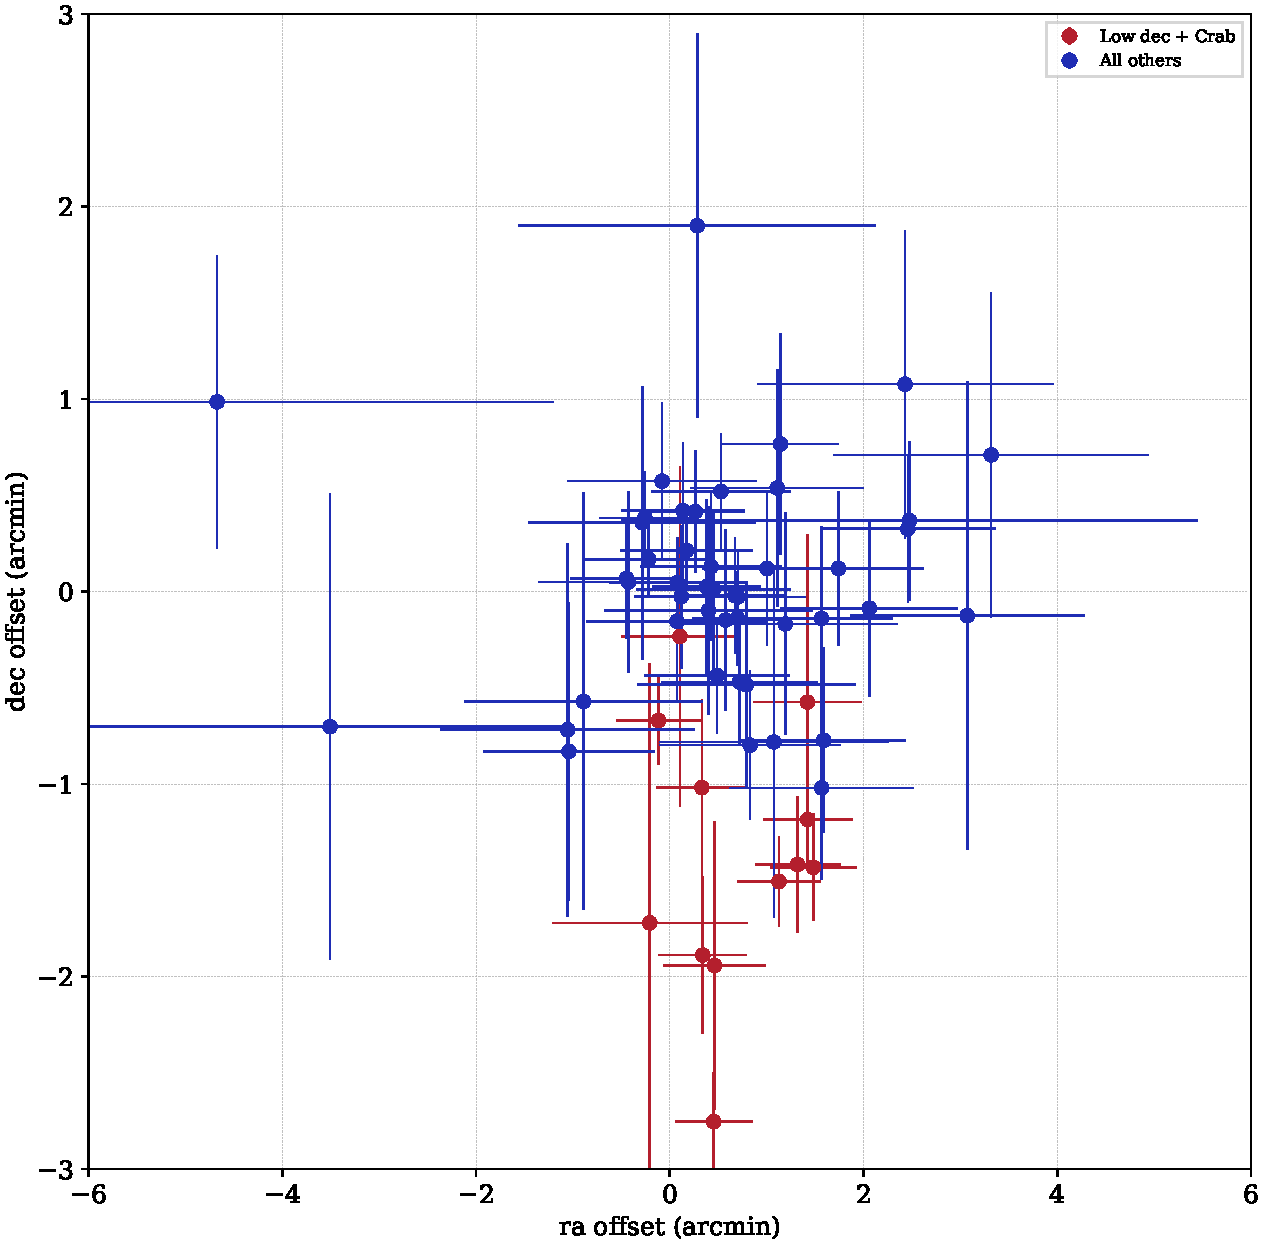
\includegraphics[width=0.33\textwidth]{figures/bb_pulsars.pdf}
%     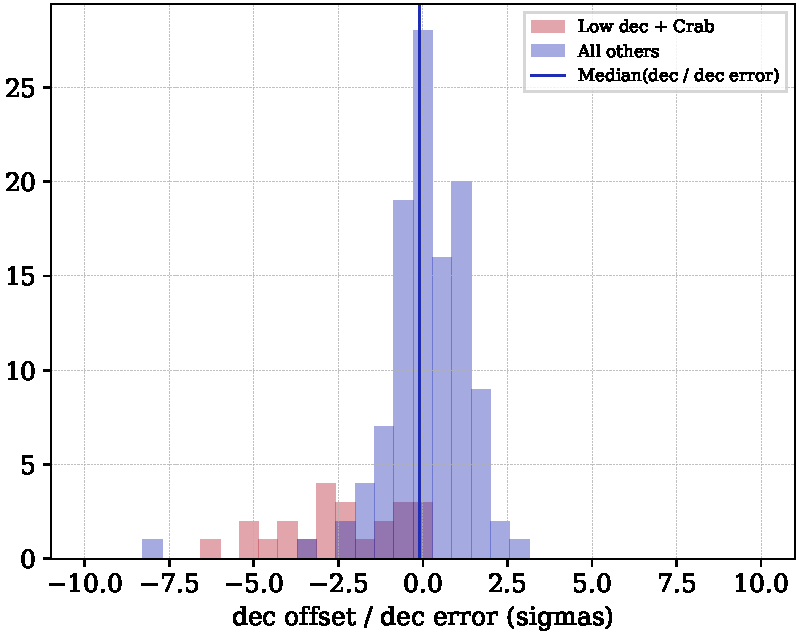
\includegraphics[width=0.33\textwidth]{figures/bb_pulsars_chisq.pdf}
%     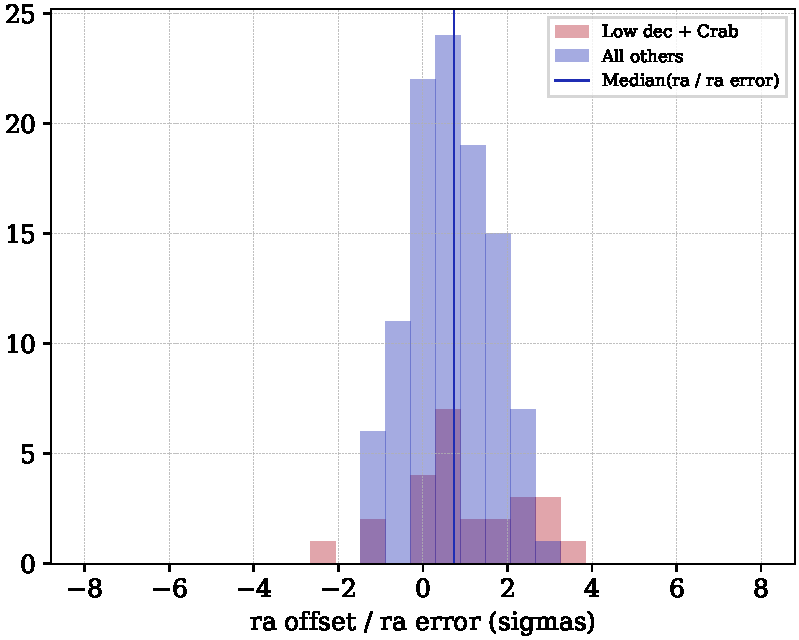
\includegraphics[width=0.33\textwidth]{figures/bb_pulsars_chisq_ra.pdf}
%     \caption{Astrometric errors for pulsars.  \textbf{TODO (Mattias?): Also plot errors versus pulsar S/N, or just bin histograms into high and low S/N samples.}}
%     \label{fig:bb_pulsars}
% \end{figure*}
\begin{figure*}
    \centering
    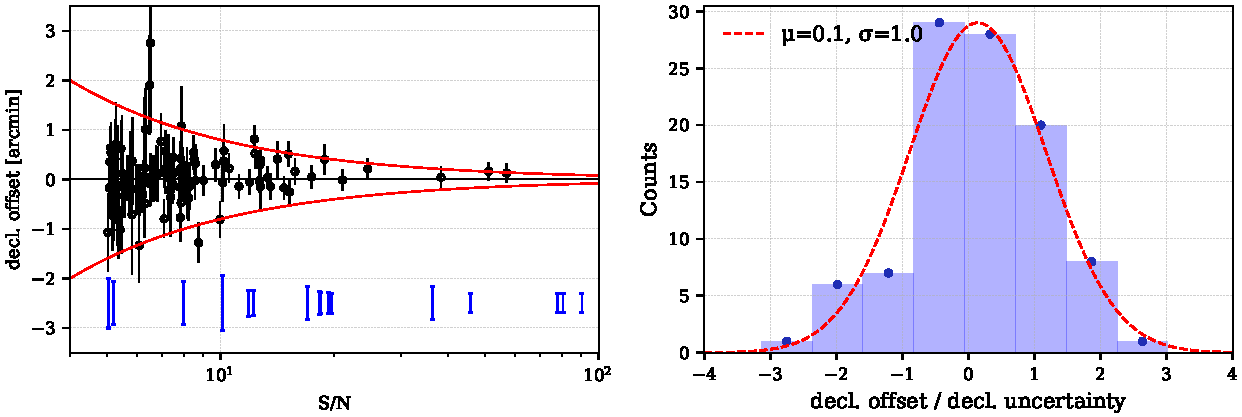
\includegraphics[width=1.0\linewidth]{figures/bblocs.pdf}
    \caption{Validation of declination uncertainties outputted by the CHIME/FRB baseband localisation pipeline \citep{michilli2020analysis}. \textit{Left panel:} Declination offsets as a function of detection S/N for a sample of 100 pulses from 18 unique pulsars covering a declination range of $+6^\circ\leq\delta\leq+80^\circ$. Offsets and their associated uncertainties are represented by open-face, black markers and errorbars, respectively. For reference, the measured S/N  and declination uncertainties associated with FRBs presented in this work are indicated by the blue errorbars at a fiducial decl. offset of $-2.5$ arcmin. \textbf{Need some high S/N pulses to test, $>$ 100 S/N}. Theoretical uncertainty for a burst detected at zenith by CHIME as a function of S/N is depicted by the two red curves \citep{michilli2020analysis}. \textit{Right:} Histogram of measured declination offsets normalized by their outputted uncertainties. As expected, the normalized values are well described by a Gaussian distribution with a mean of 0.1 and standard deviation of 1.0 (overplotted dashed, red line).}
    \label{fig:bb_pulsars}
\end{figure*}
VLBI localization: discuss calibrator choice – \textbf{TODO: Make figure showing example field.}


\subsection{Minor-axis localization using VLBI}
Along the east-west direction, the position is strongly constrained by VLBI localization. Following the basic strategy of~\citep{leung2020synoptic}, we use the full-array baseband dumps to search for bright ($\sim\SI{1}{\jansky}$) VLBI calibrators from the RFC and VLBA catalogs within the baseband dump, whose effective field of view on the sky is $\sim \SI{200}{\deg^2}$. At each station, we formed station beams towards each of the $\sim 200$ VLBI calibrators within the field of view. Following~\citep{andrew2024calibrator}, we placed a single correlator pointing in each station beam, and each pointing was correlated using the~\texttt{PyFX} correlator~\citep{leung2024vlbi}. Visibilities were saved if the calibrator was detected. We detected up to 15 VLBI calibrators per baseband dump this way.

Selecting the closest calibrator minimizes the impact of ionospheric and beam variations, but choosing the brightest calibrator can ensure a more robust detection. In both strategies, we could accidentally choose a calibrator that is impacted by an unknown systematic, such as those detected in a sidelobe or confused sources. Since we expect all sources to be affected by similar total instrumental delay, we can mitigate this risk by comparing the delays of all calibrators in the field and identify outliers. We thus adopt the following strategy for calibrator selection --- for all calibrators detected in the field, select those whose measured total delays are within 2~ns of the median delay. From these, choose the calibrator closest in declination to the baseband localization of the FRB.

To compare this with other strategies, we perform localizations using all available calibrators for a set of known pulsars, and compare the offsets of the measured to true positions. Figure~\ref{fig:psr_cal_test} shows the offsets for a set of between 1 and 5 observations of 18 pulsars. Each column of points represents a single observation (i.e., baseband dump), with each point the result of localizing using a different in-beam calibrator. The colored points indicate the results of using the calibrator chosen with each selection criterion -- ``Closest \& Good'' refers to the strategy described in the last paragraph, while ``S/N'' and ``Closest'' refer to using the calibrator with the highest S/N cross-correlation and the closest calibrator in declination, respectively.

For almost all of the calibrators tested, our chosen selection method (green points) ensures offsets are less than 2.5 arcsec.

% For each event, we plot the measured position offset using the calibrator selected with three strategies -- ``Closest \& Good'' refers to the strategy described in the last paragraph, while ``S/N'' and ``Closest'' refer to using the calibrator with the highest S/N cross-correlation and the closest calibrator in declination, respectively. In some cases, two or more strategies selected the same calibrator.

\begin{figure*}
	\centering
	
\includegraphics[width=1.01\linewidth]{{figures/pulsar_cal_offset_compare}.png}
	\caption{Offsets of measured from true positions, along the baseline direction, for a sample of pulsars. Each point is the offset of the measured position from the true position using a different in-beam calibrator. Each column shows offsets for a given baseband acquisition, grouped by target pulsar. The color of the point indicates which calibrator would be selected by each selection strategy -- red for maximum S/N, blue for the closest in declination, and green for our chosen strategy of selecting the closest calibrator that is ``in-family'' with the others.}
	\label{fig:psr_cal_test}
\end{figure*}



%\textbf{Figure (Adam?): VLBI accuracy for pulsars versus target-calibrator separation and target brightness.} This motivate our minor axis ellipse dimensions, which for conservatism and simplicity we assume to be a constant 2 (sometimes 3) nanoseconds.

\section{Host Association}\label{sec:association}
We use the default priors in the PATH formalism to assign posterior probabilities to each catalogued galaxy allowed by the combined localization region from baseband and CHIME-KKO VLBI. Each localization region is cross-matched with a widefield galaxy survey. Where possible (20/100 fields), we cross-match against the Dark Energy Camera Legacy Survey (DECaLS) to find a host galaxy. In the remainder of fields, we use imaging from Pan-STARRS PS1, which covers the entire CHIME/FRB discovery footprint. 

The galaxies overlapping the localization region are vetted for contamination by misclassified stars, and posterior probabilities $P(O|x)$ are assigned to each galaxy. With a properly-calibrated $P(U)$ for each galaxy survey, the posterior probabilities rank each galaxy in order of the probability of being the true host. A prior of $P(U) = 0.1$ was chosen for fields which overlapped widefield imaging from the DECaL Survey, while a prior of $P(U) = 0.2$ was chosen for PanSTARRS-PS1 fields.
\textbf{Figure: 2D histogram of $P(O|x)$ versus $z$ for all (even empty) fields; put good HG in a different color. Also do the same but as a function of DM instead of $z$.}


Fig.~\ref{fig:hg_images} shows host galaxies with high posterior probabilities (decide on cutoff). Because CHIME's discovery footprint is entirely contained within the footprint of Pan-STARRS, We display publicly-available host galaxy images from Pan-STARRS DR1 to maintain uniformity across the sample.

\subsection{Unseen/ambiguous FRB hosts}
Any FRB detector will have to contend with FRBs with no readily-detected host galaxy. This can suggest a high-redshift origin for these FRB if the localization region is sufficiently small to make a robust association at faint optical magnitudes, as shown in Marnoch 2024. In our case, the localization ellipses are of size 70-600 square arcseconds, which only allows for a robust association out to a limiting magnitude of $\sim 20$, as seen by the gold-standard associations in our sample.

FRBs with small localizations with no optically-detected host galaxy in multi-wavelength cross-matching.


\begin{figure*}[h]
    \centering
    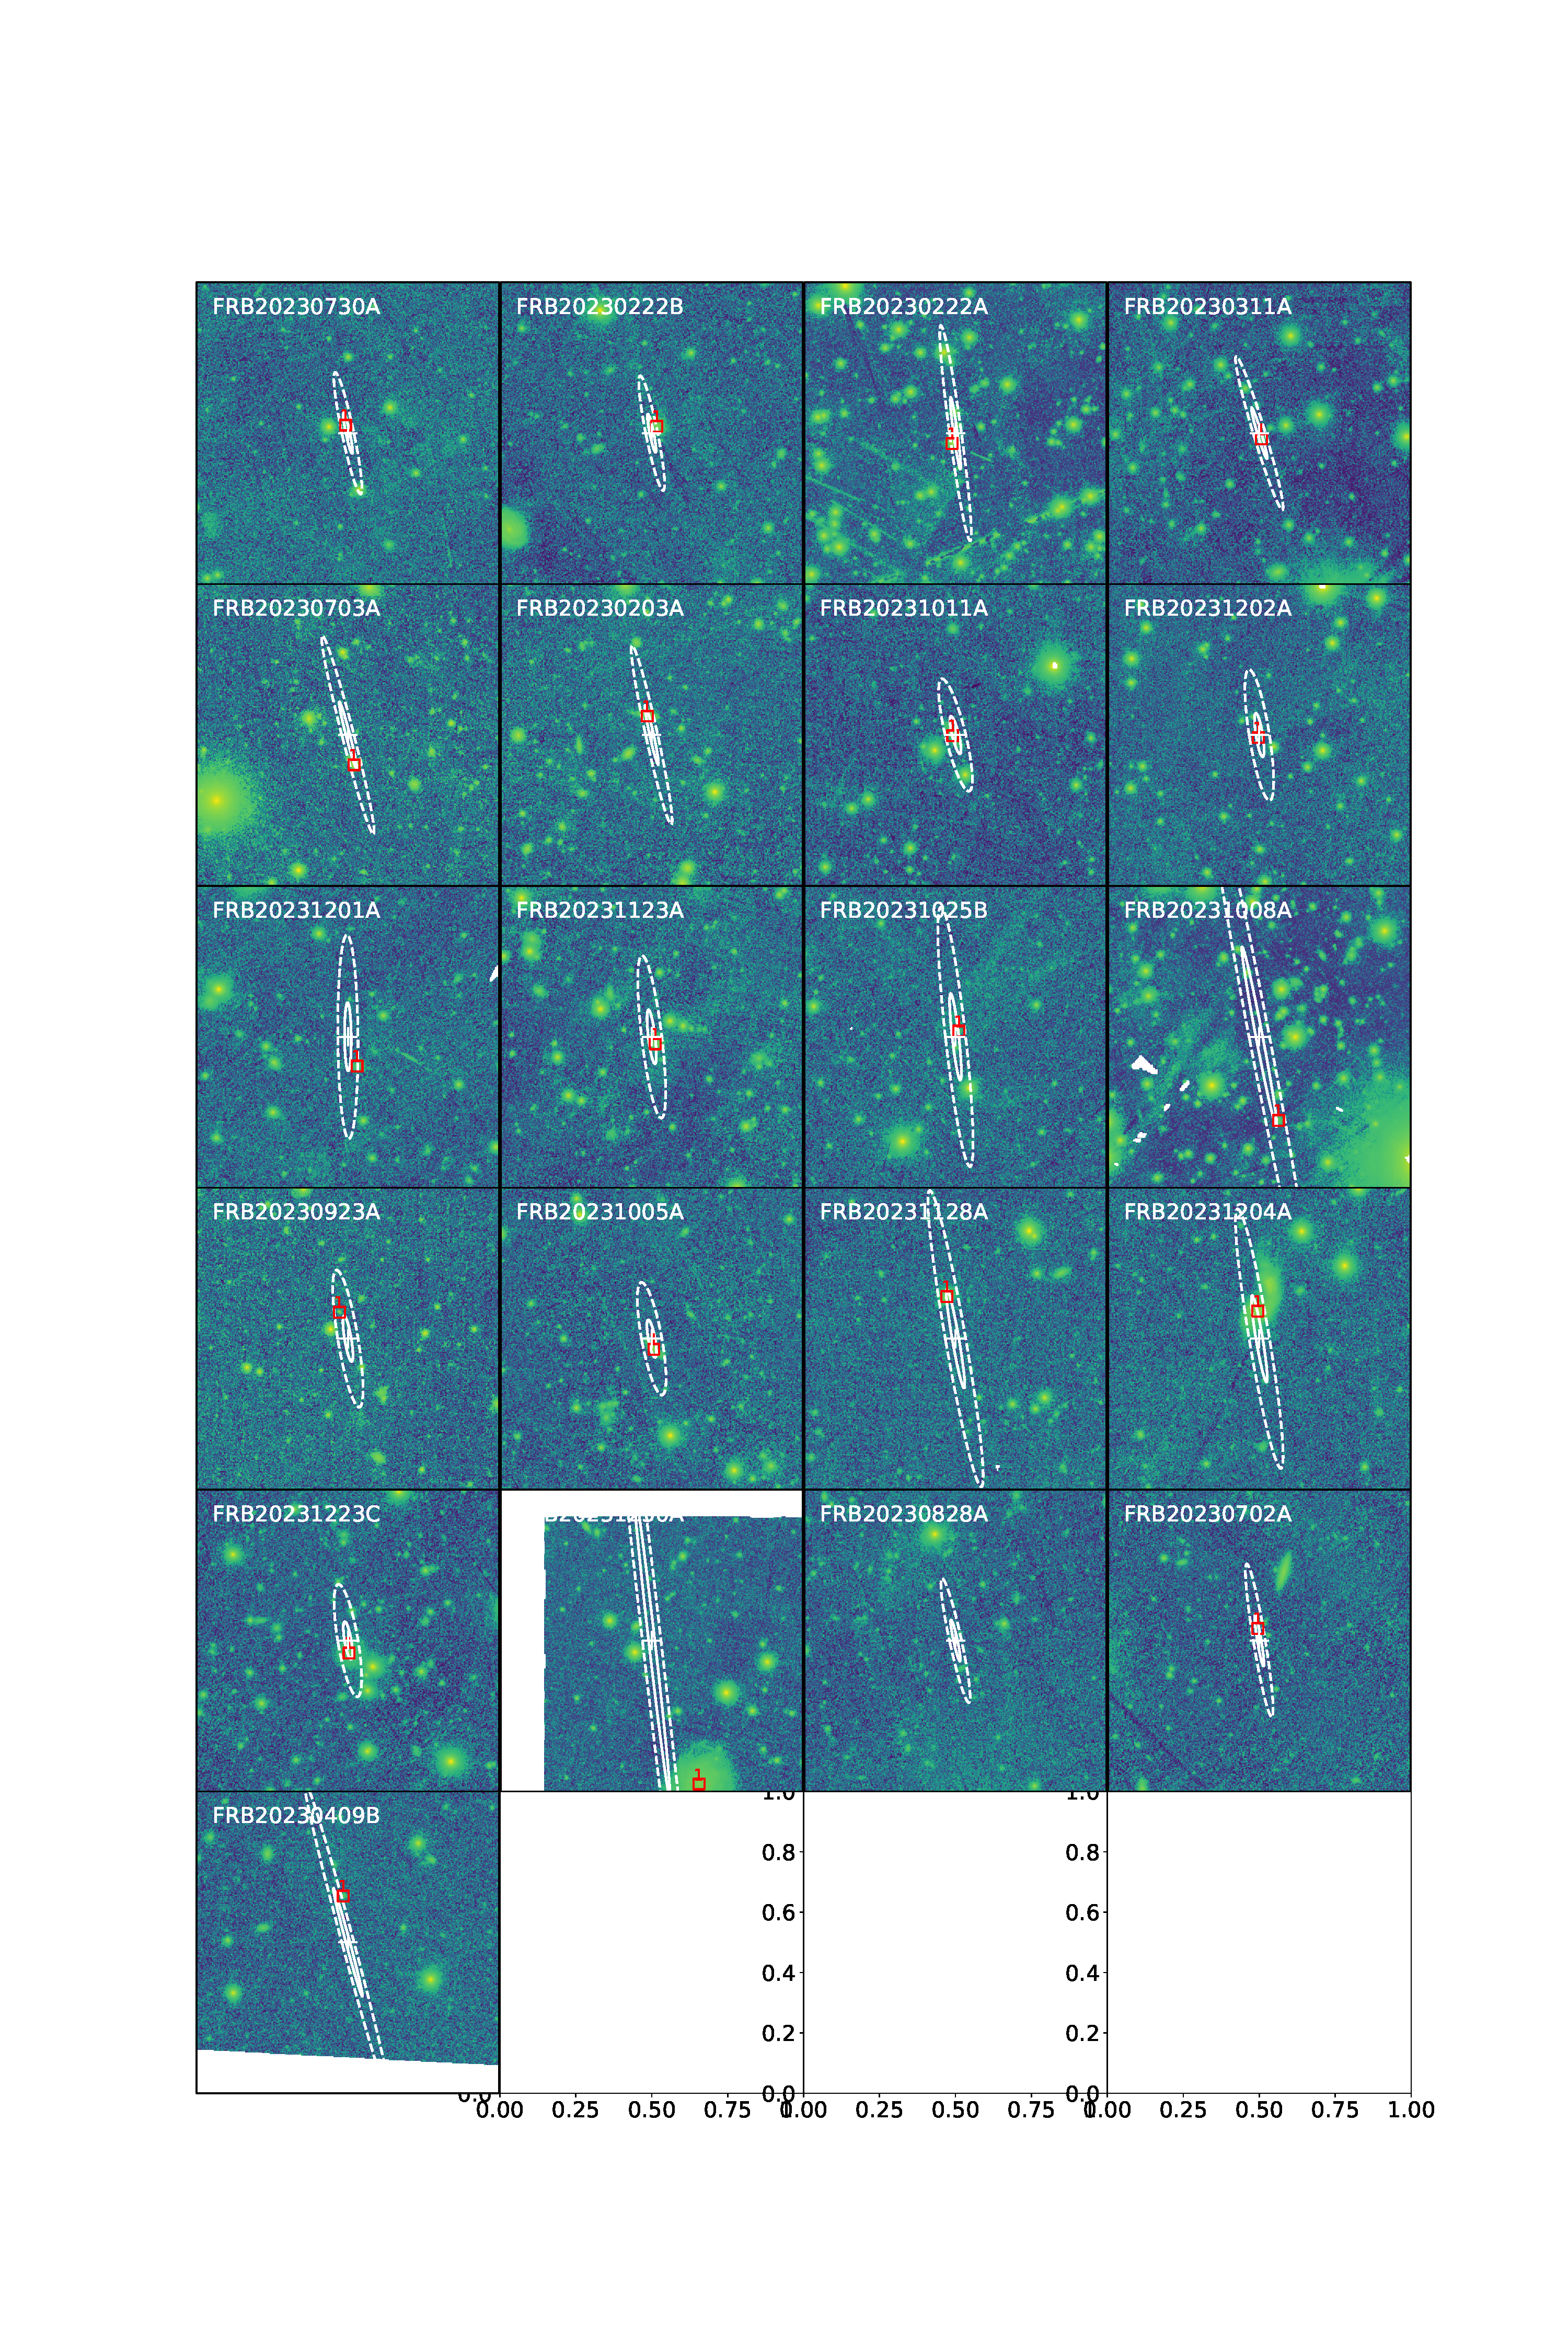
\includegraphics[width=0.9\textwidth]{figures/hg_images.pdf}
    \caption{All of our host galaxies. \textbf{TODO: TNS names in lower RHS; dark background; zoom in on hosts. Need volunteer to help with this (perhaps somebody from F4 or with PATH experience? Discuss: should we have a separate figure with zoom-in on hosts?)}}
    \label{fig:hg_images}
\end{figure*}

\begin{figure*}[h]
    \centering
    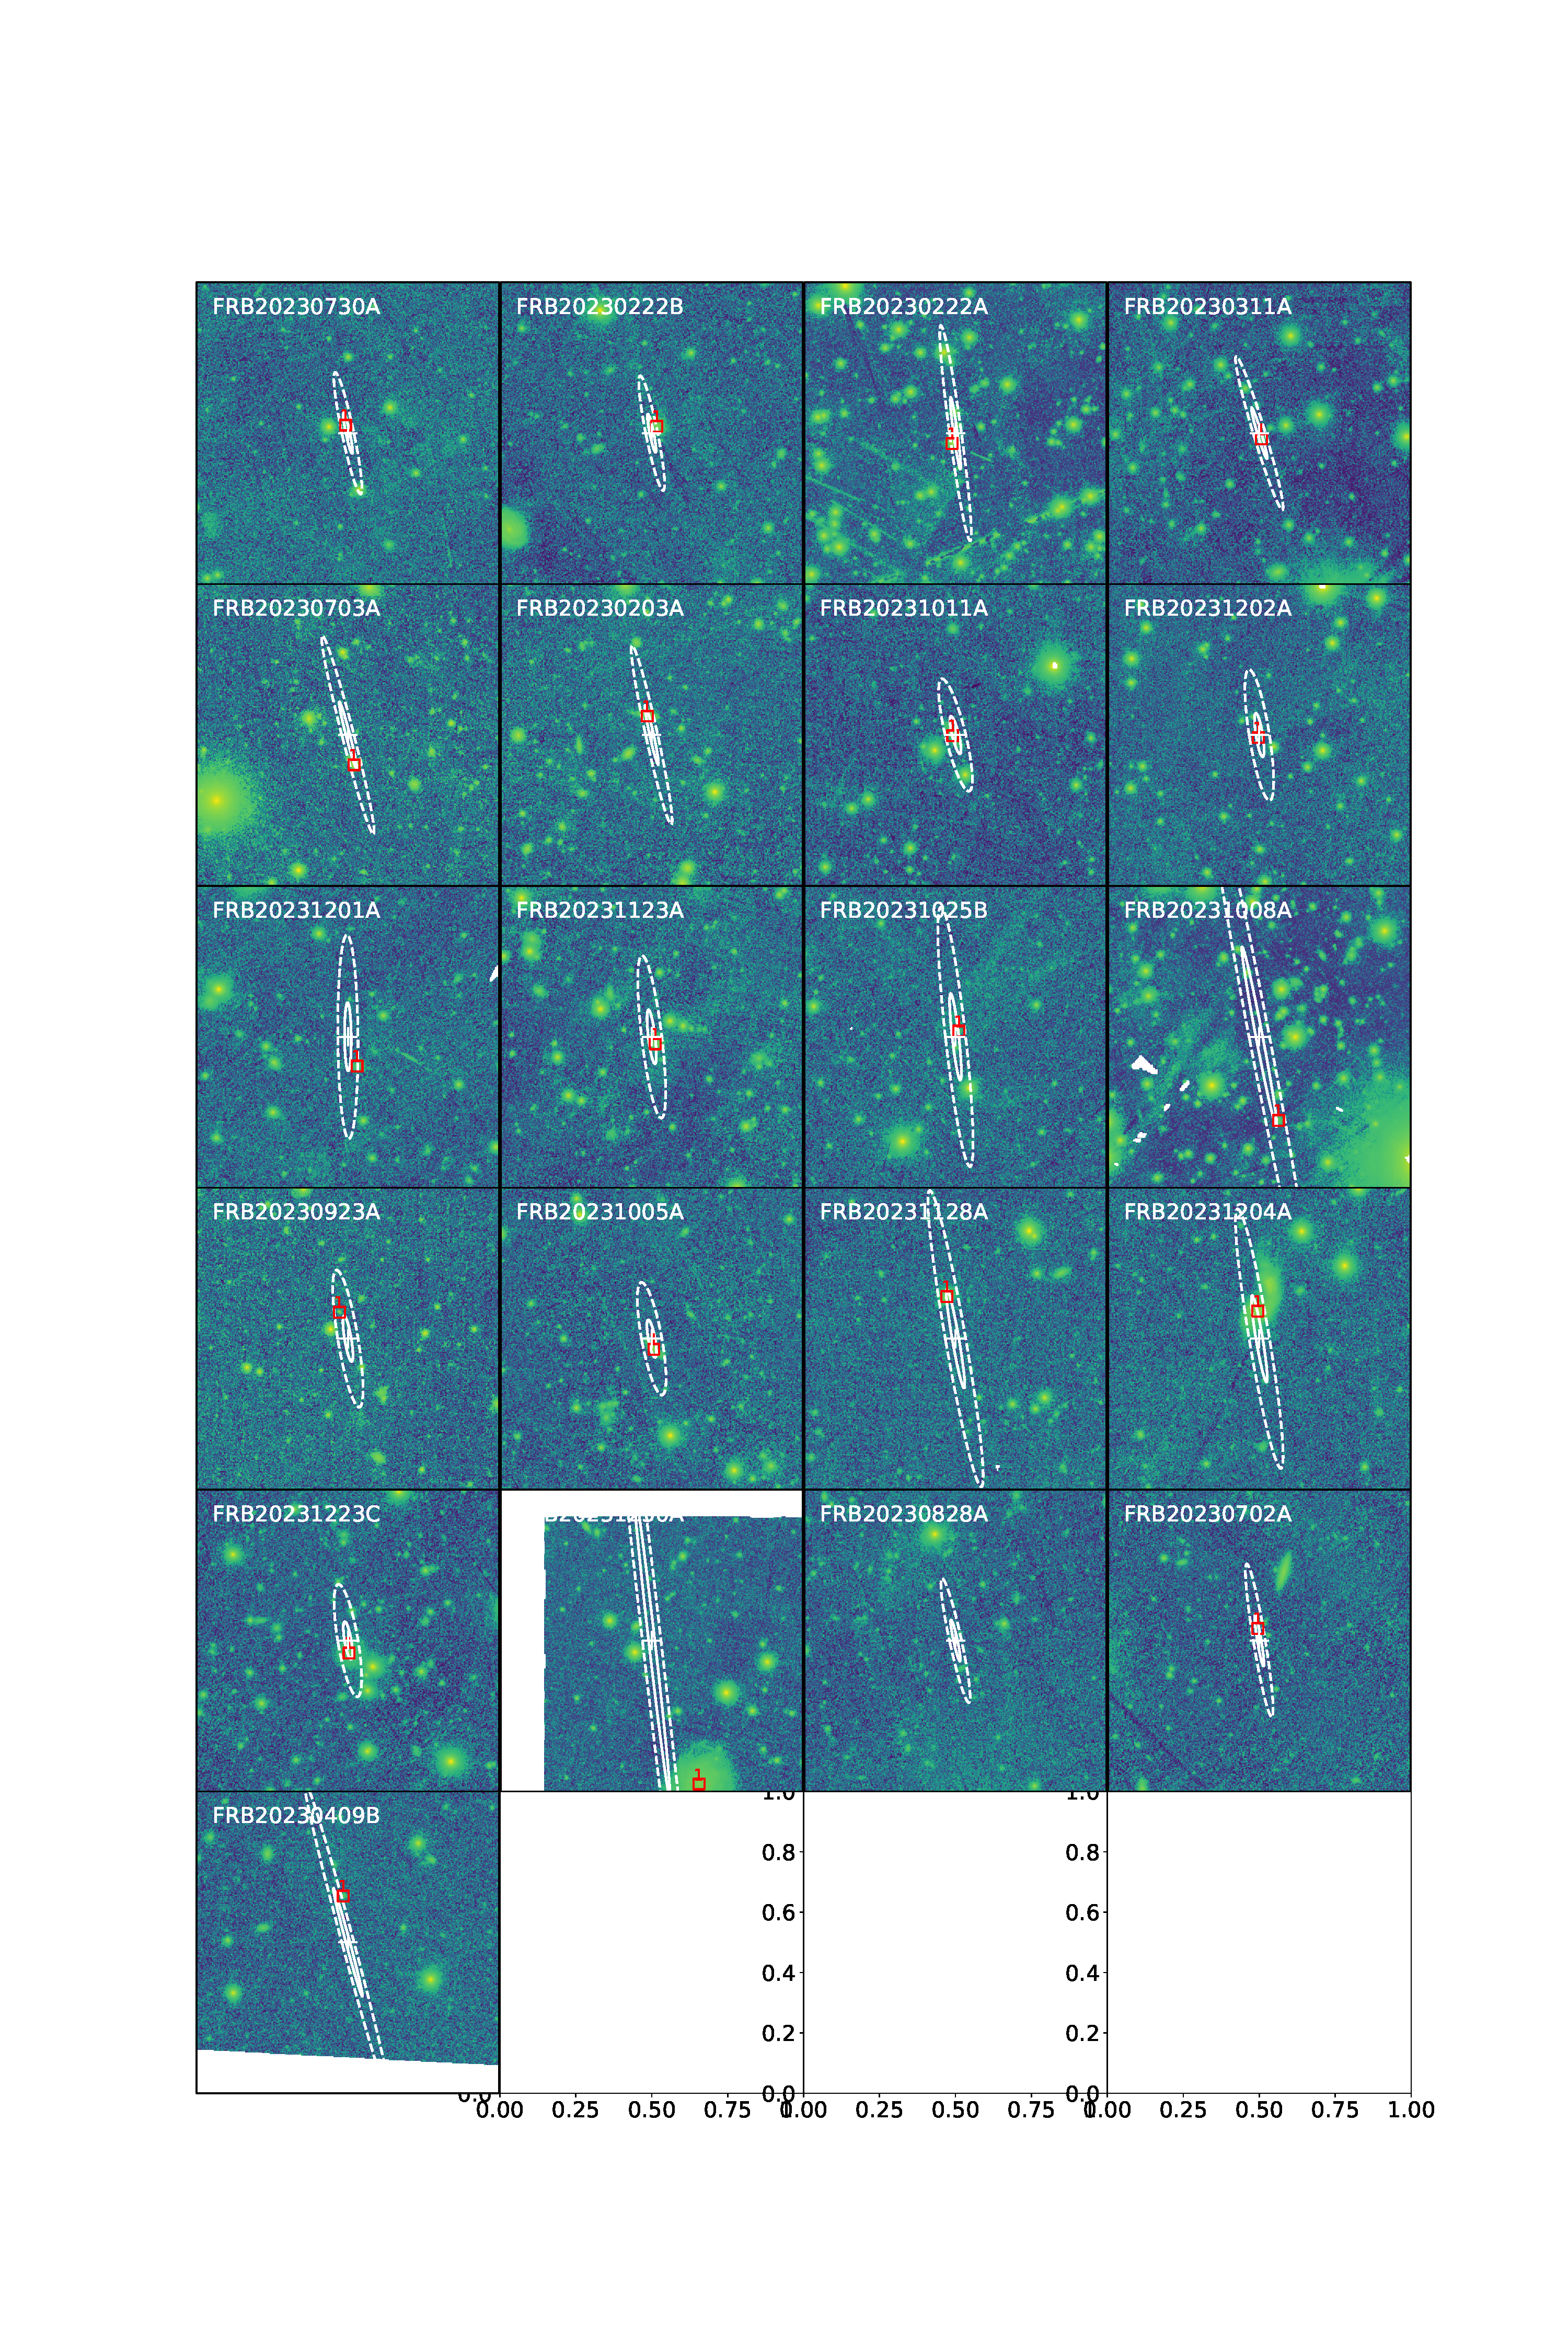
\includegraphics[width=0.9\textwidth]{figures/hg_images.pdf}
    \caption{All of our host galaxies. \textbf{TODO: TNS names in lower RHS; dark background; zoom in on hosts. Need volunteer to help with this (perhaps somebody from F4 or with PATH experience? Discuss: should we have a separate figure with zoom-in on hosts?)}}
    \label{fig:hg_images}
\end{figure*}

The morphology of these bursts is rich. All Stokes-I waterfall plots in baseband data are shown in Fig.~\ref{fig:waterfalls}. To check for morphological differences in FRB dynamic spectra, we have ordered the dynamic spectra in decreasing order of energy implied by their putative host redshifts, but we defer detailed morphological fitting for later work. We calculate the flux and fluence of these bursts to directly measure their energies.

\begingroup
\setlength{\tabcolsep}{1pt}
\begin{figure*}
\begin{tabular}{cccc}
\centering
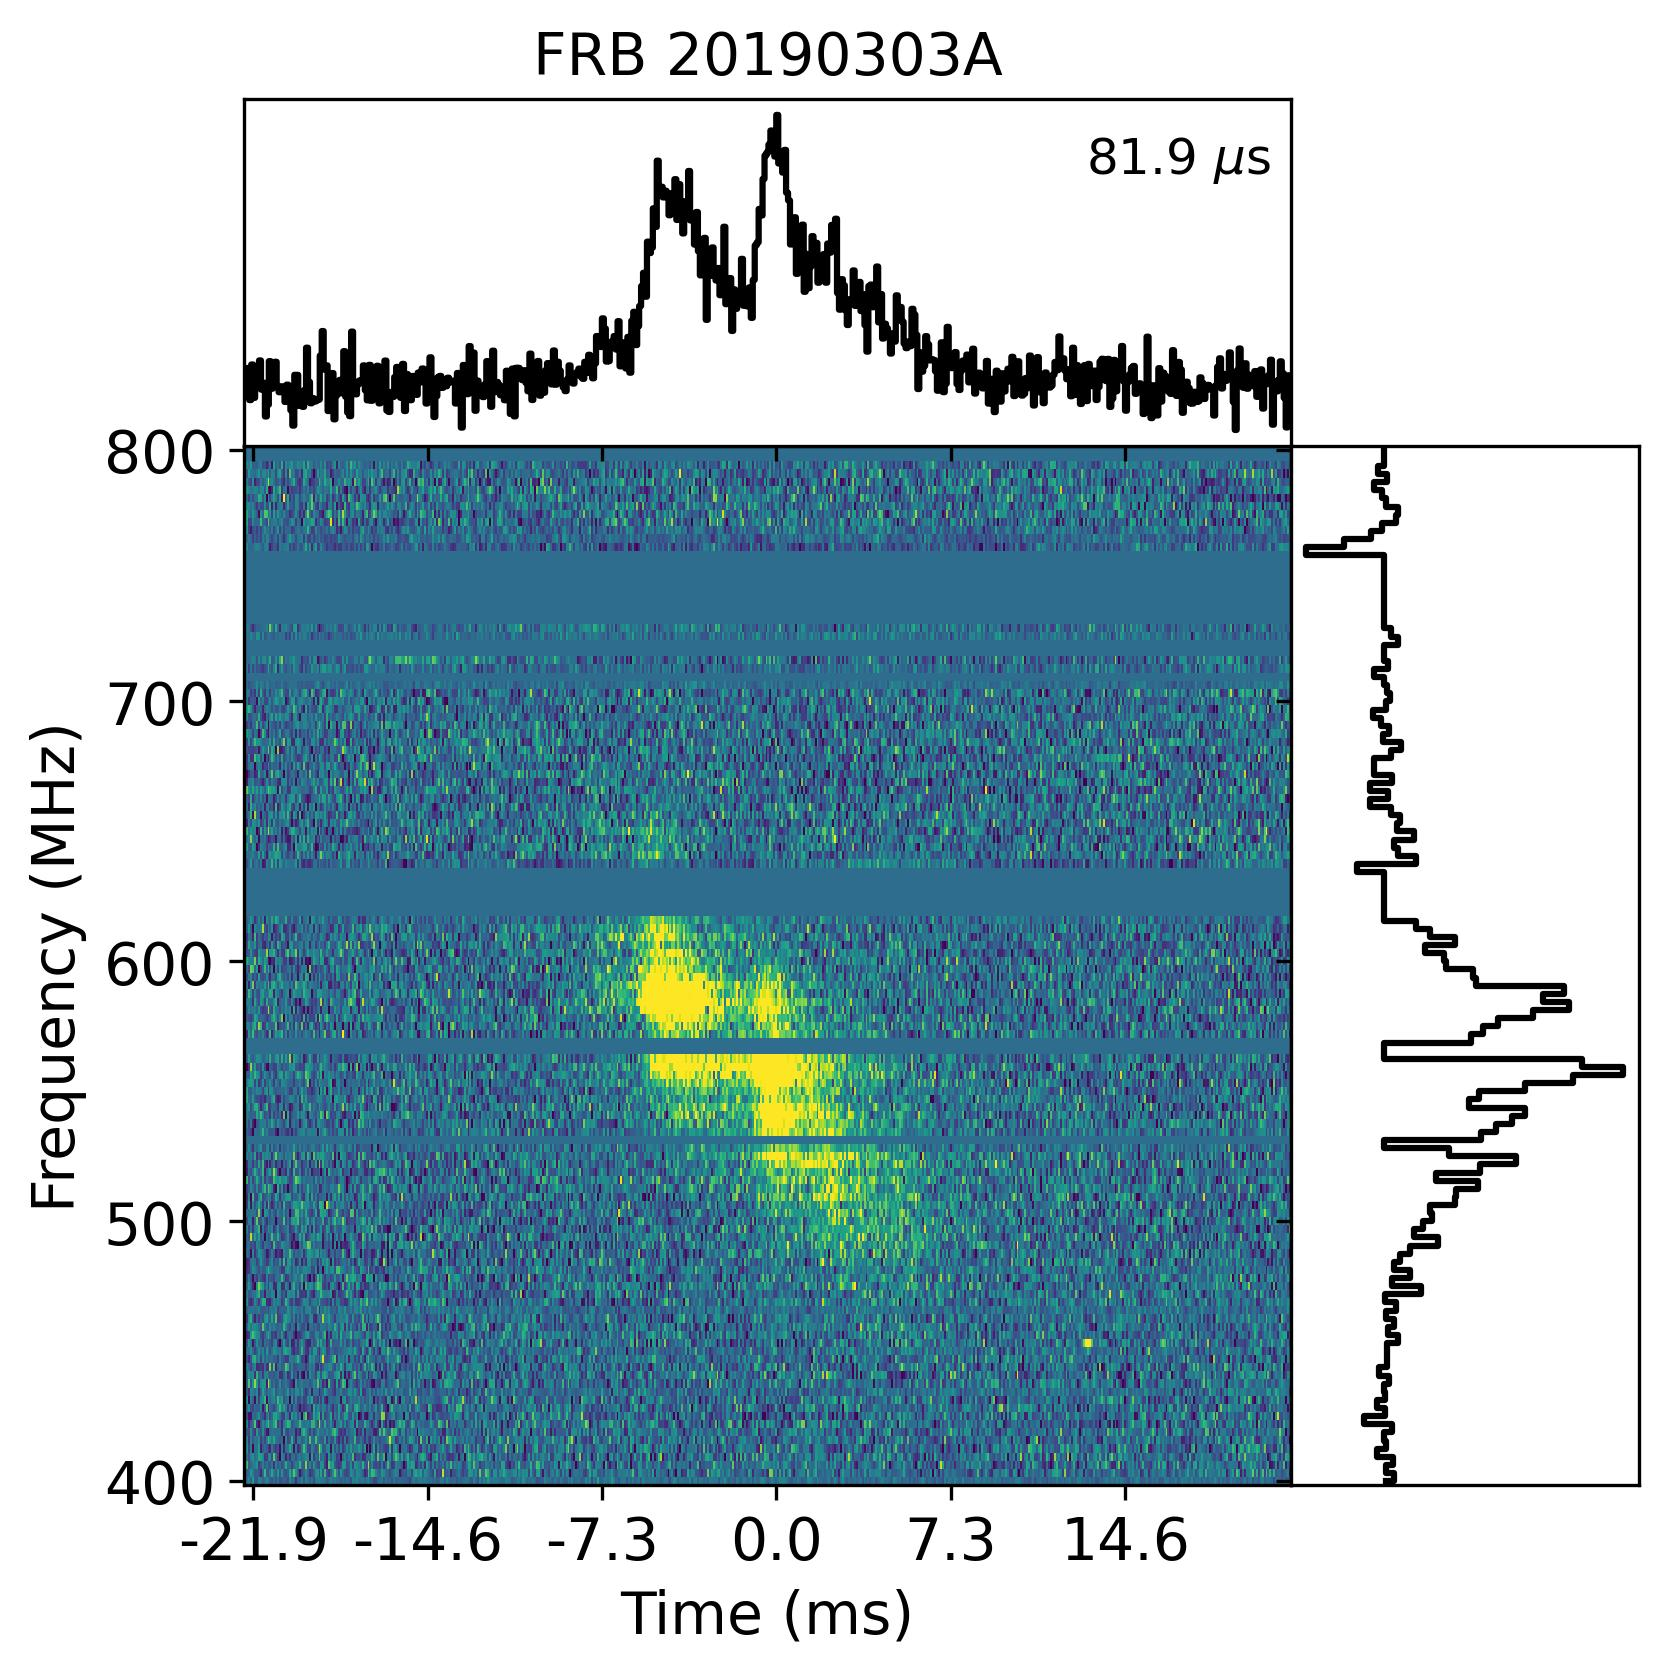
\includegraphics[width = 0.22\textwidth]{figures/FRB 20190303A_wfall.jpg} &
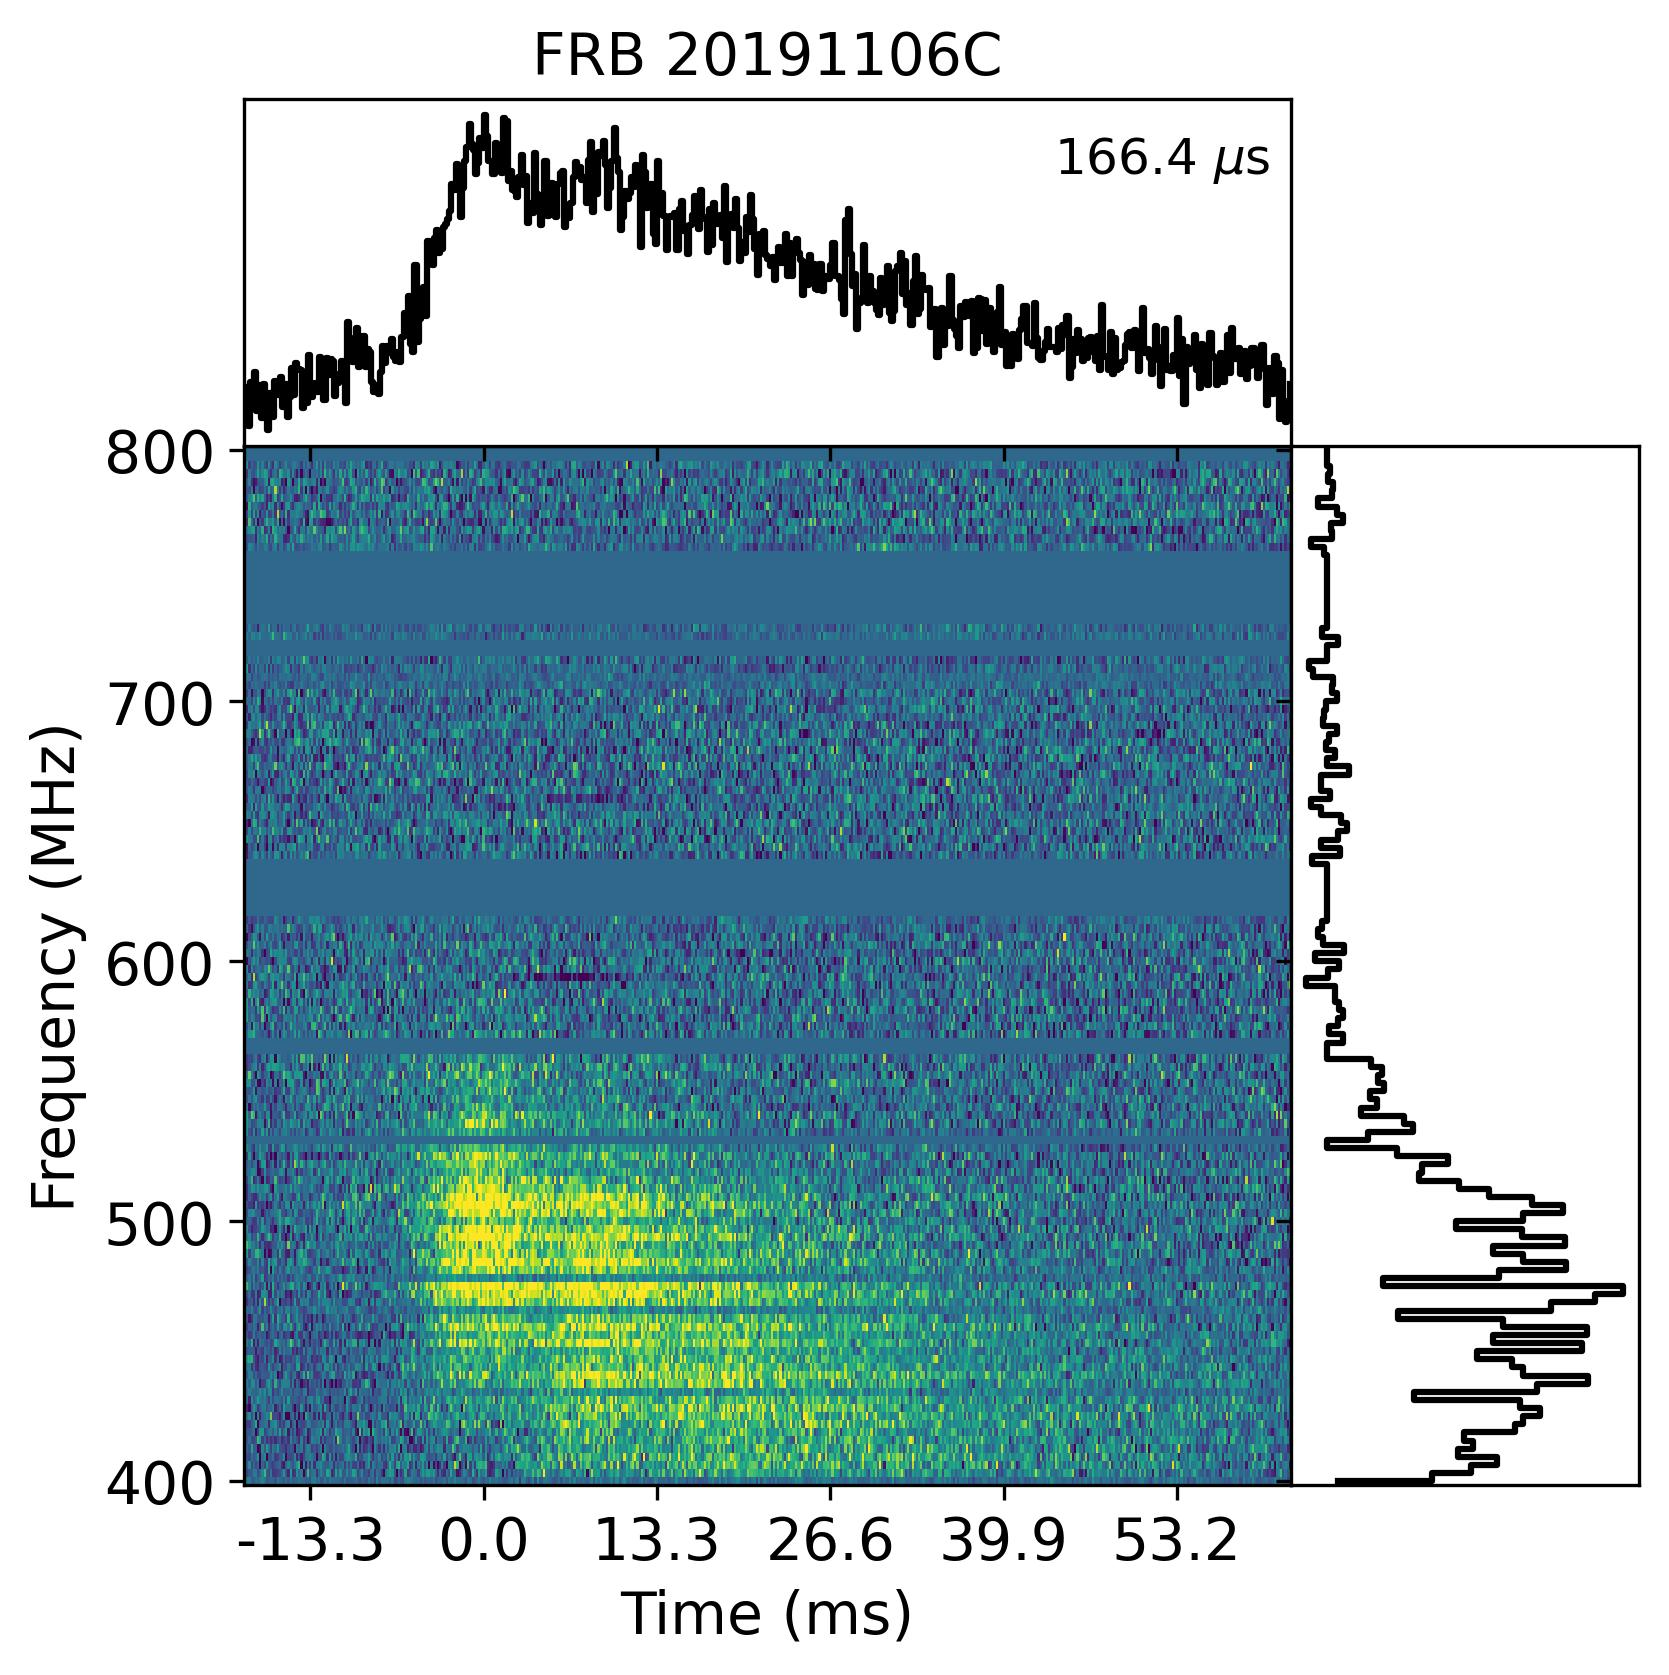
\includegraphics[width = 0.22\textwidth]{figures/FRB 20191106C_wfall.jpg} &
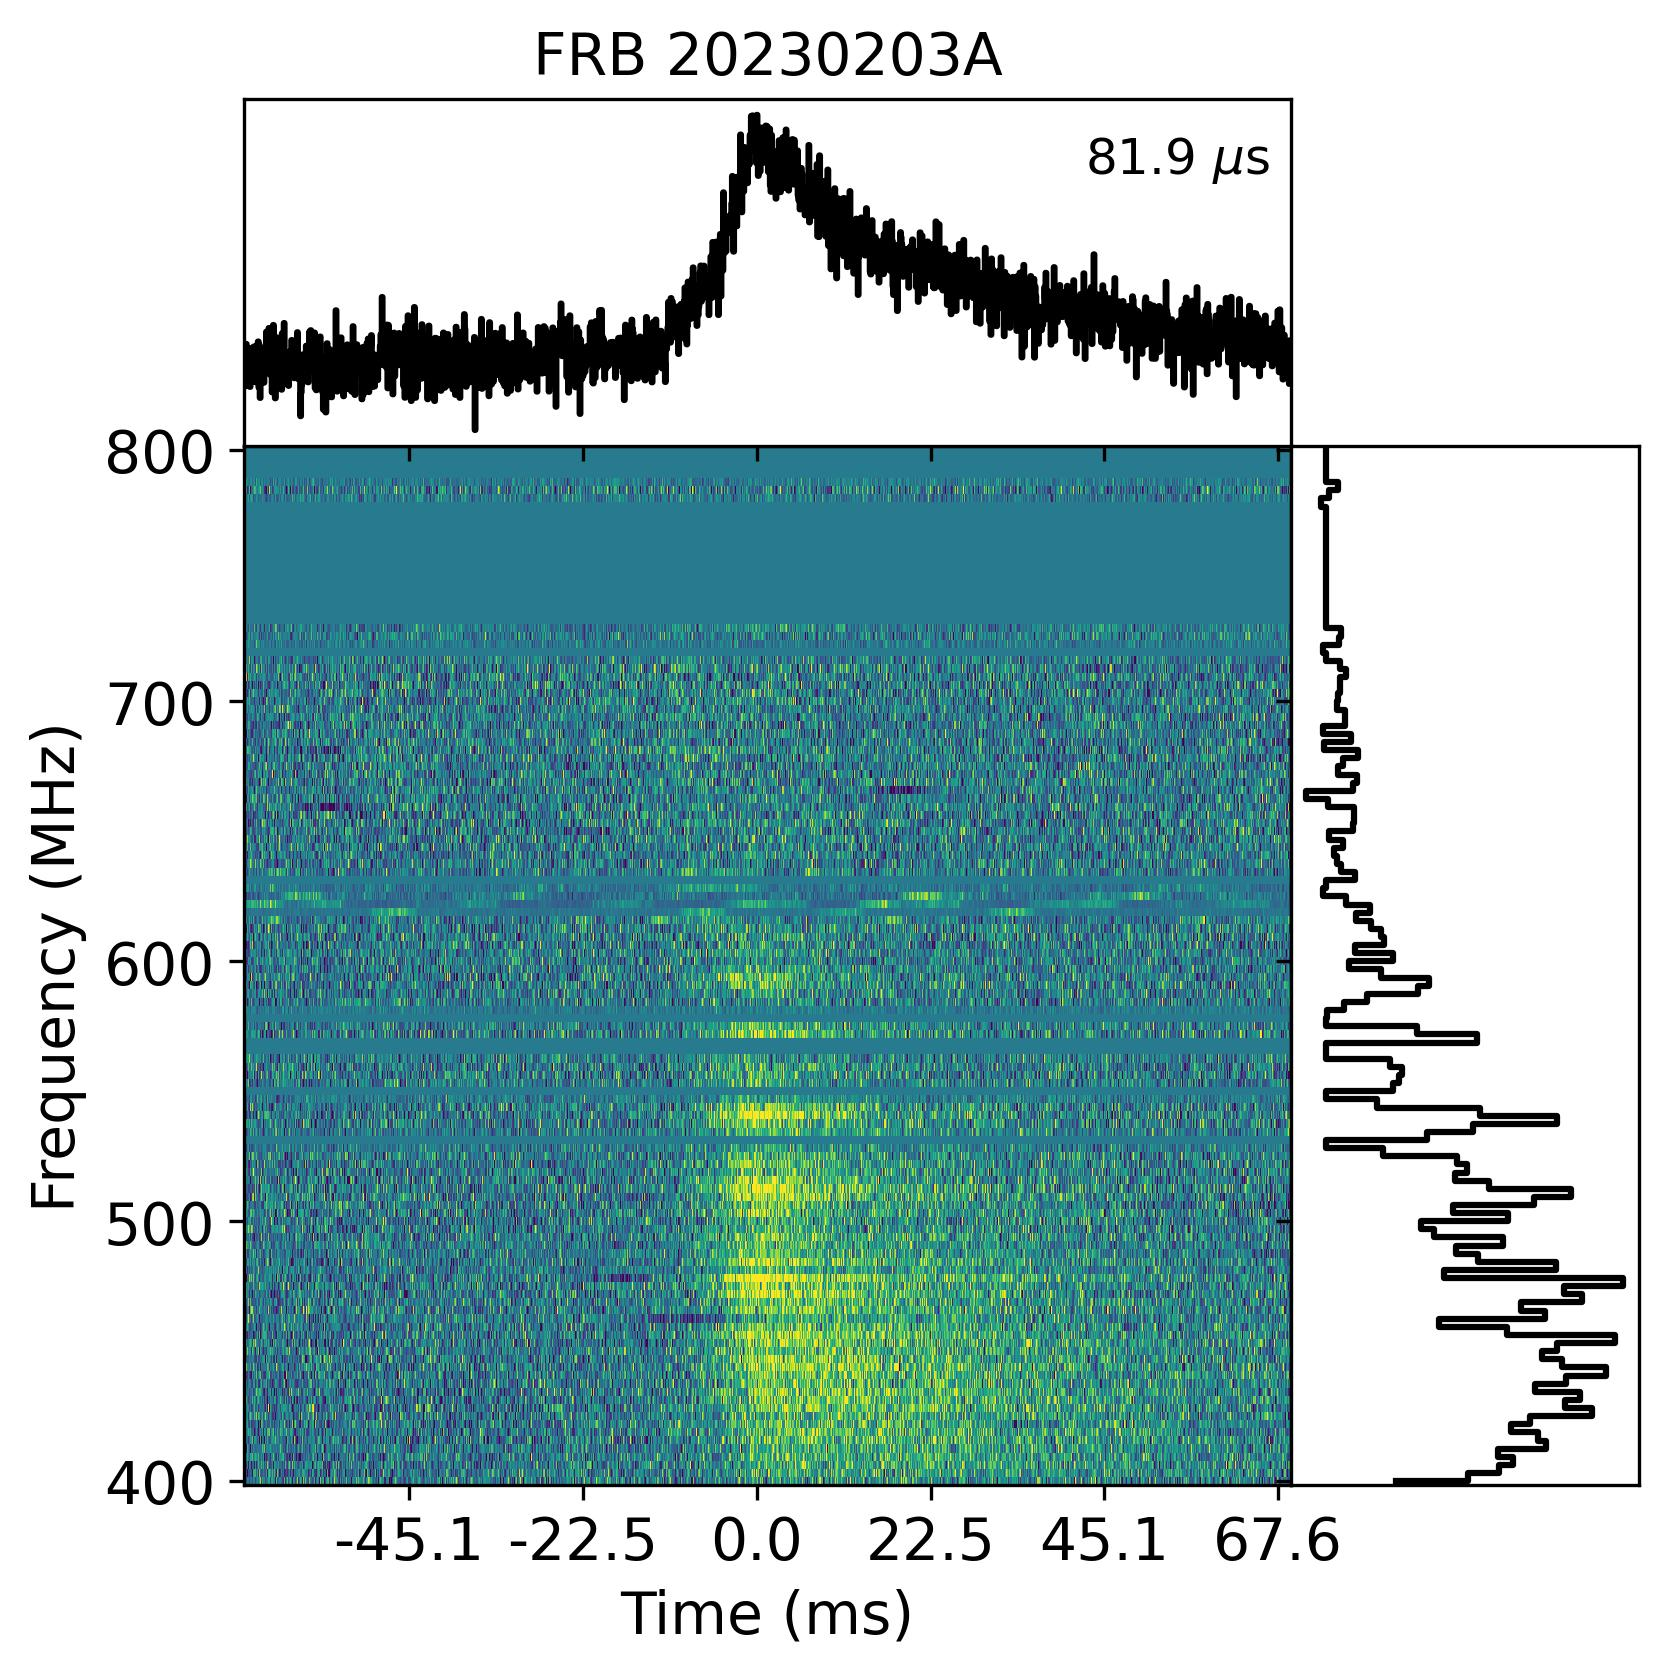
\includegraphics[width = 0.22\textwidth]{figures/FRB 20230203A_wfall.jpg} &
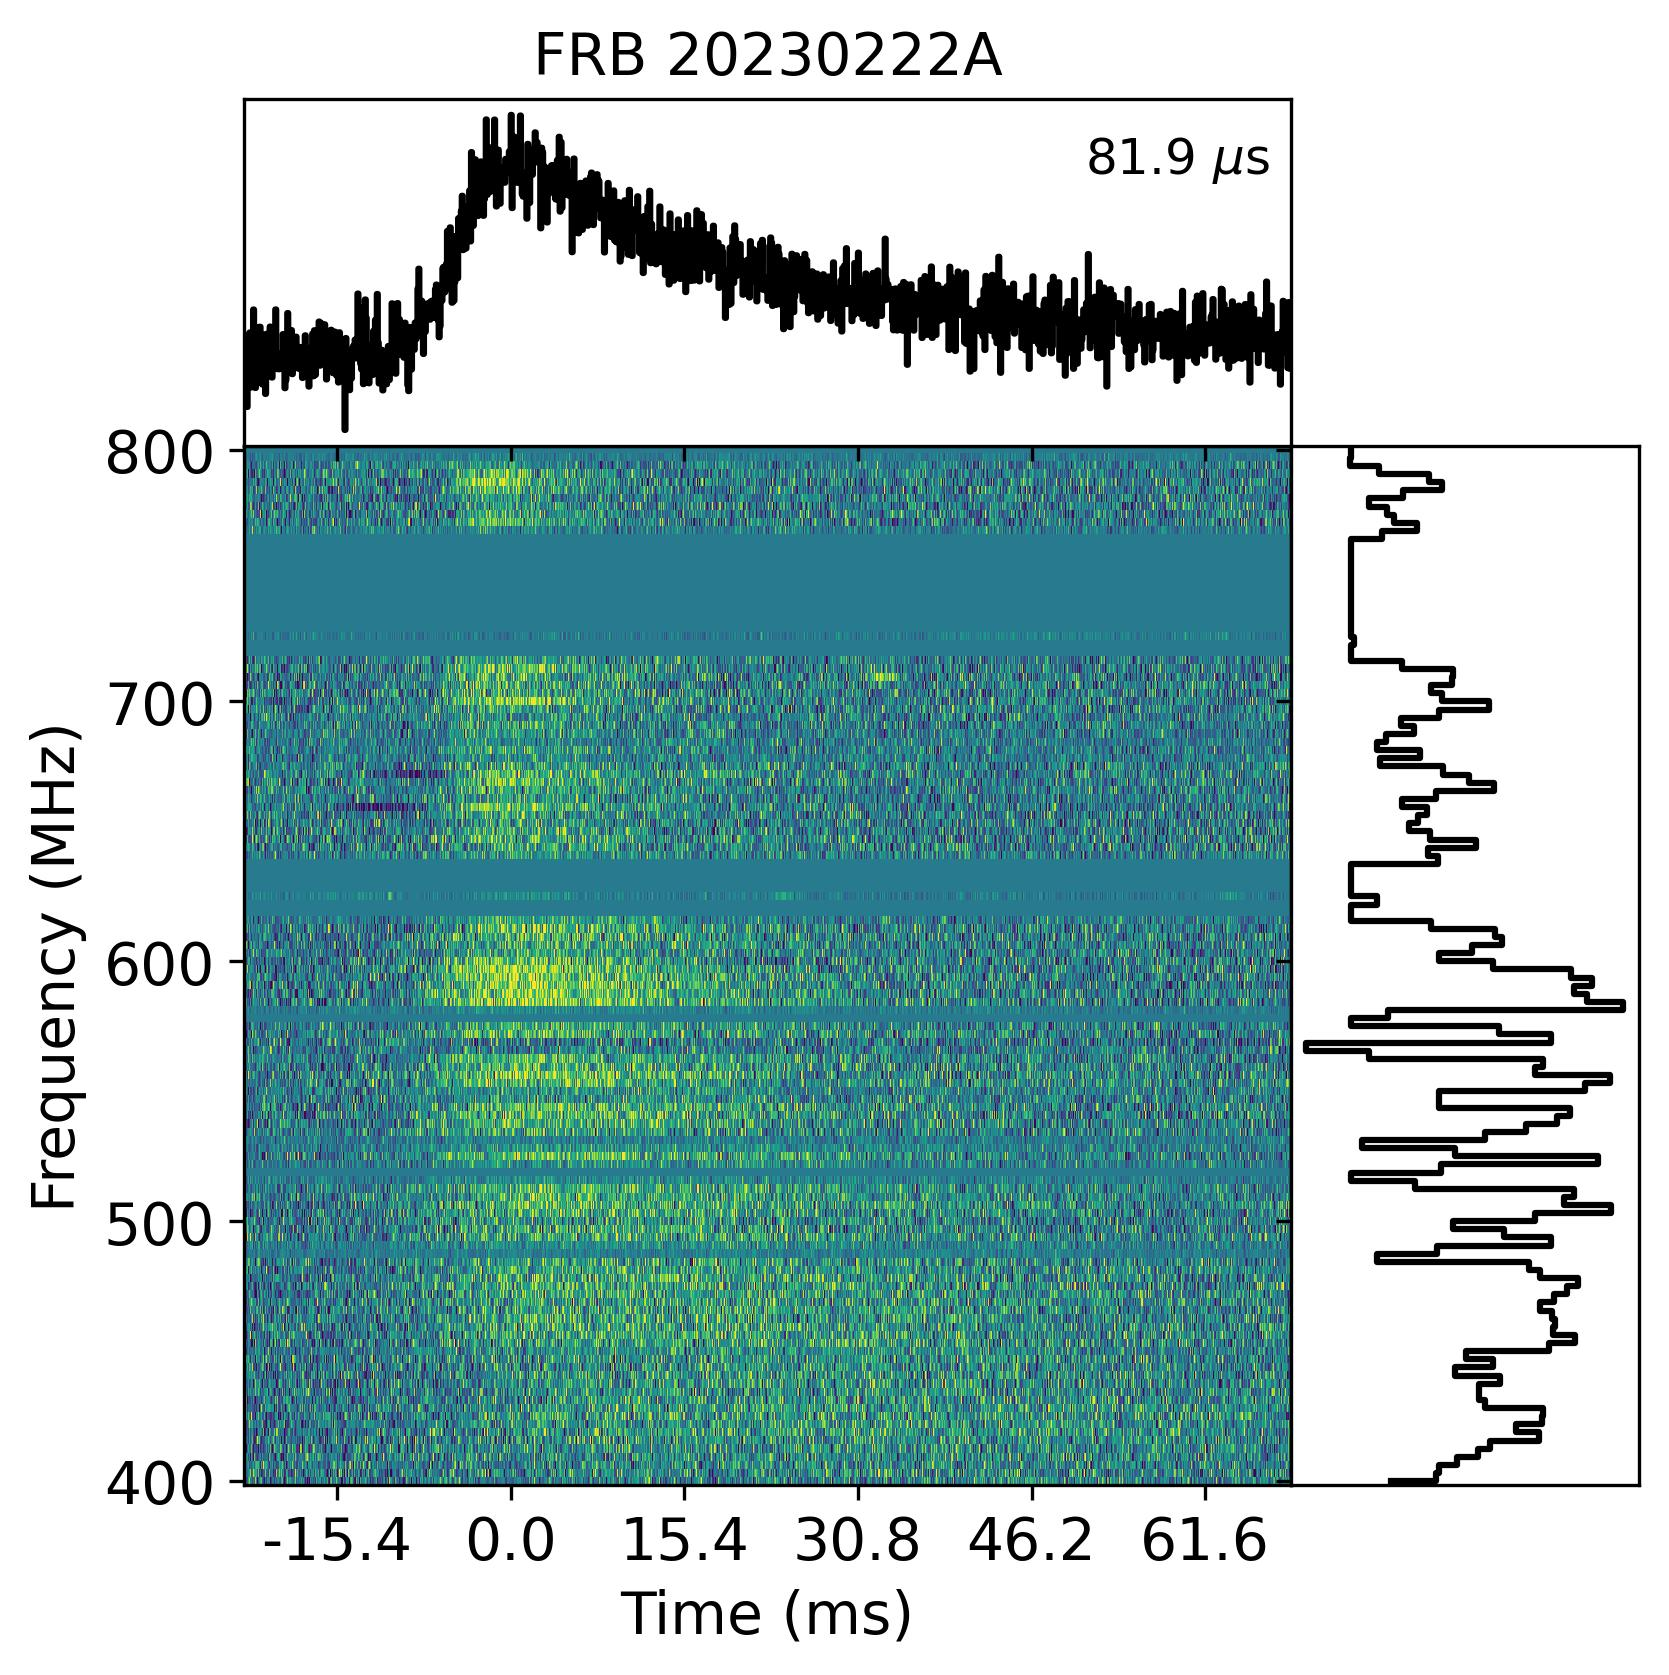
\includegraphics[width = 0.22\textwidth]{figures/FRB 20230222A_wfall.jpg} \\
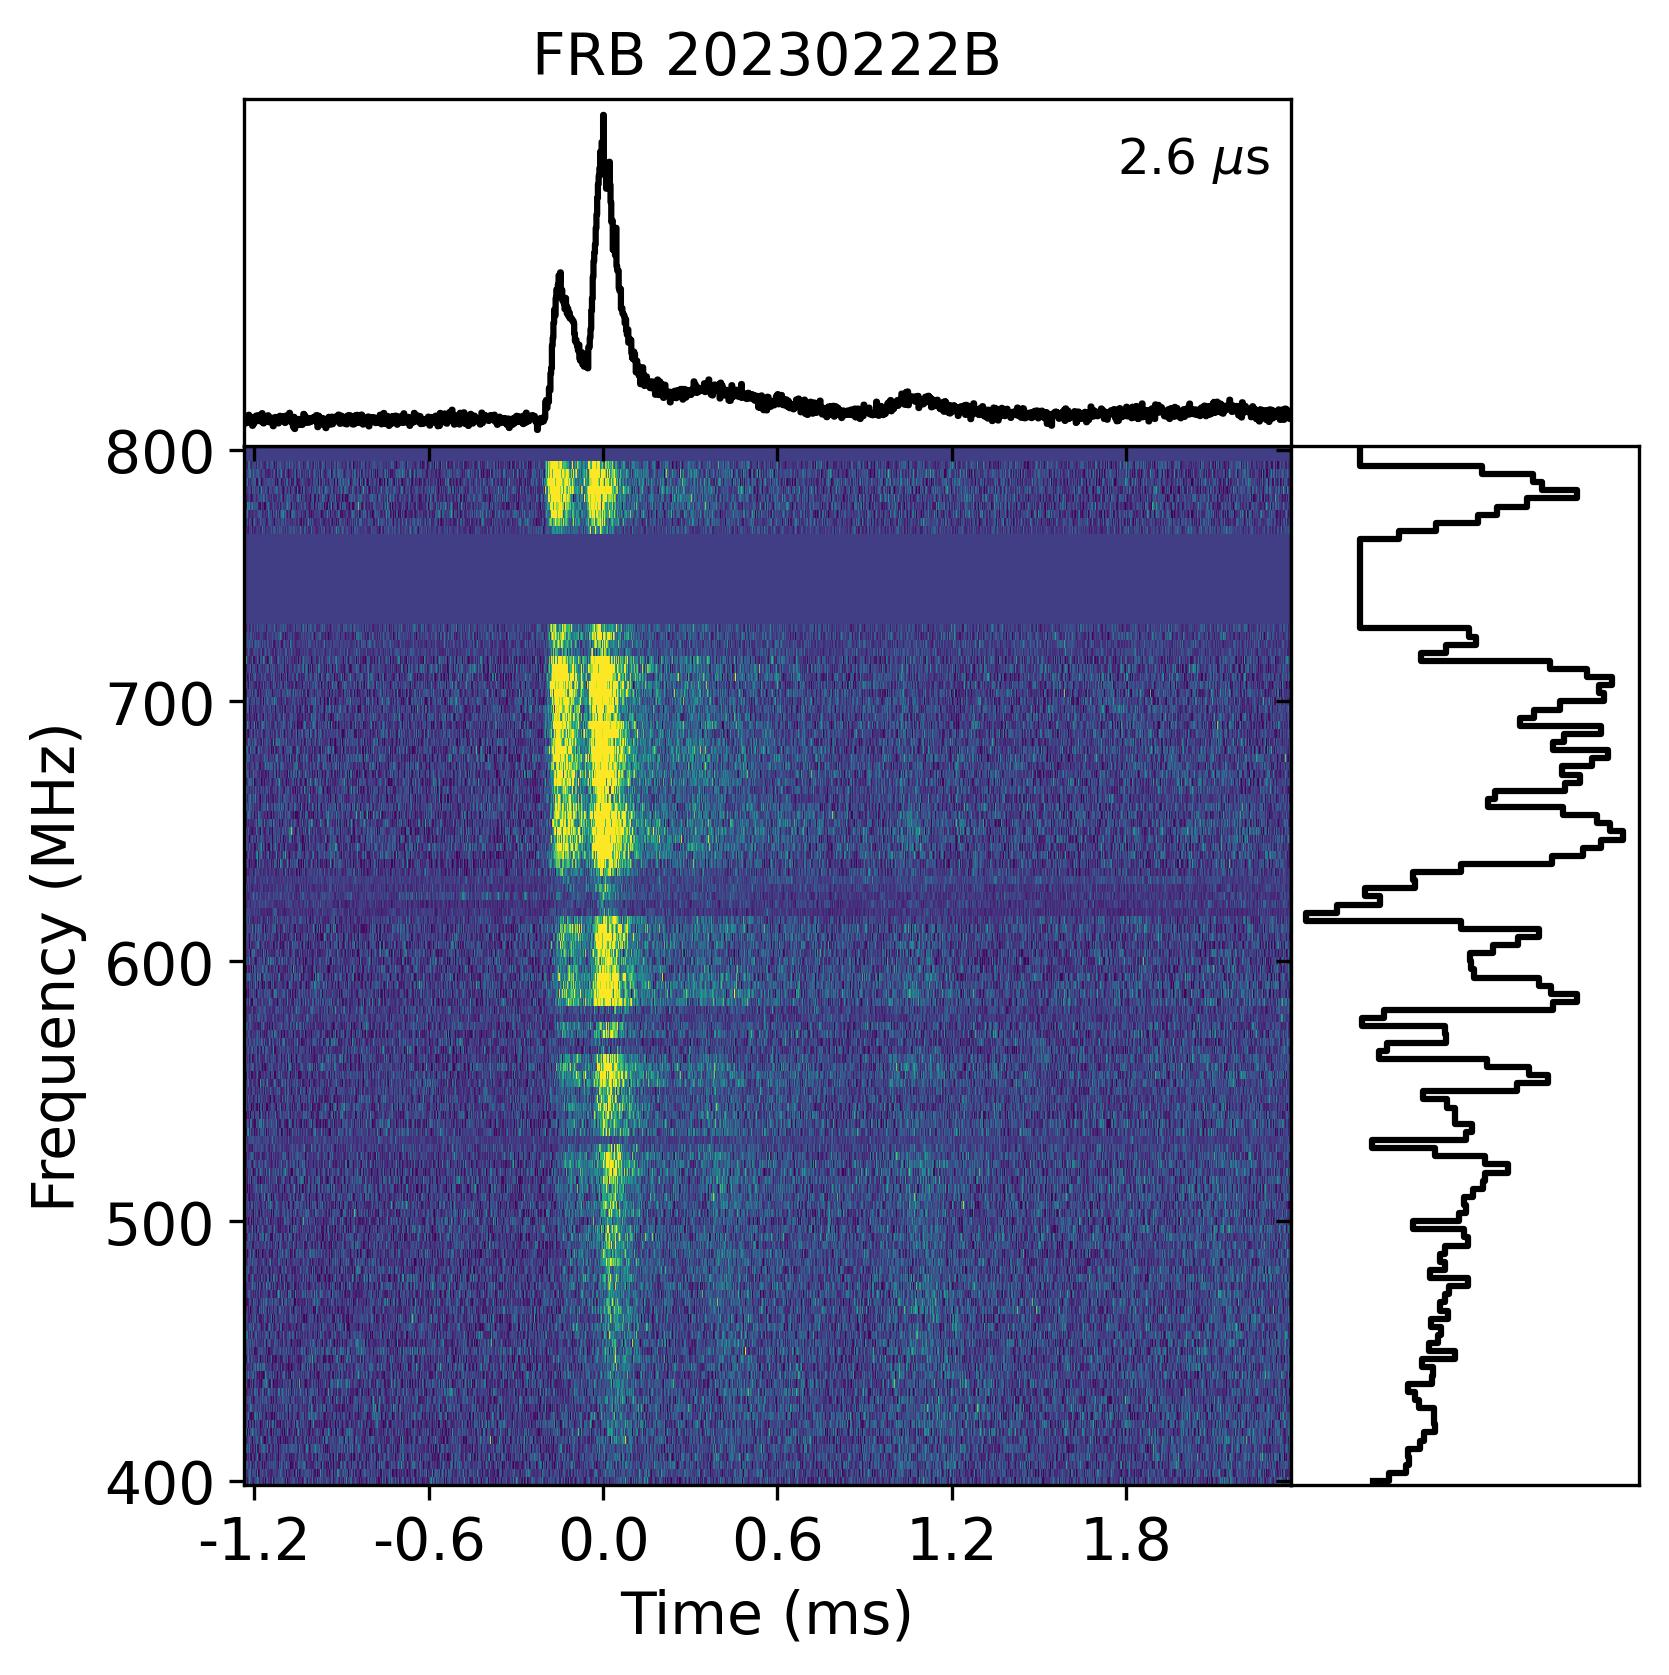
\includegraphics[width = 0.22\textwidth]{figures/FRB 20230222B_wfall.jpg} &
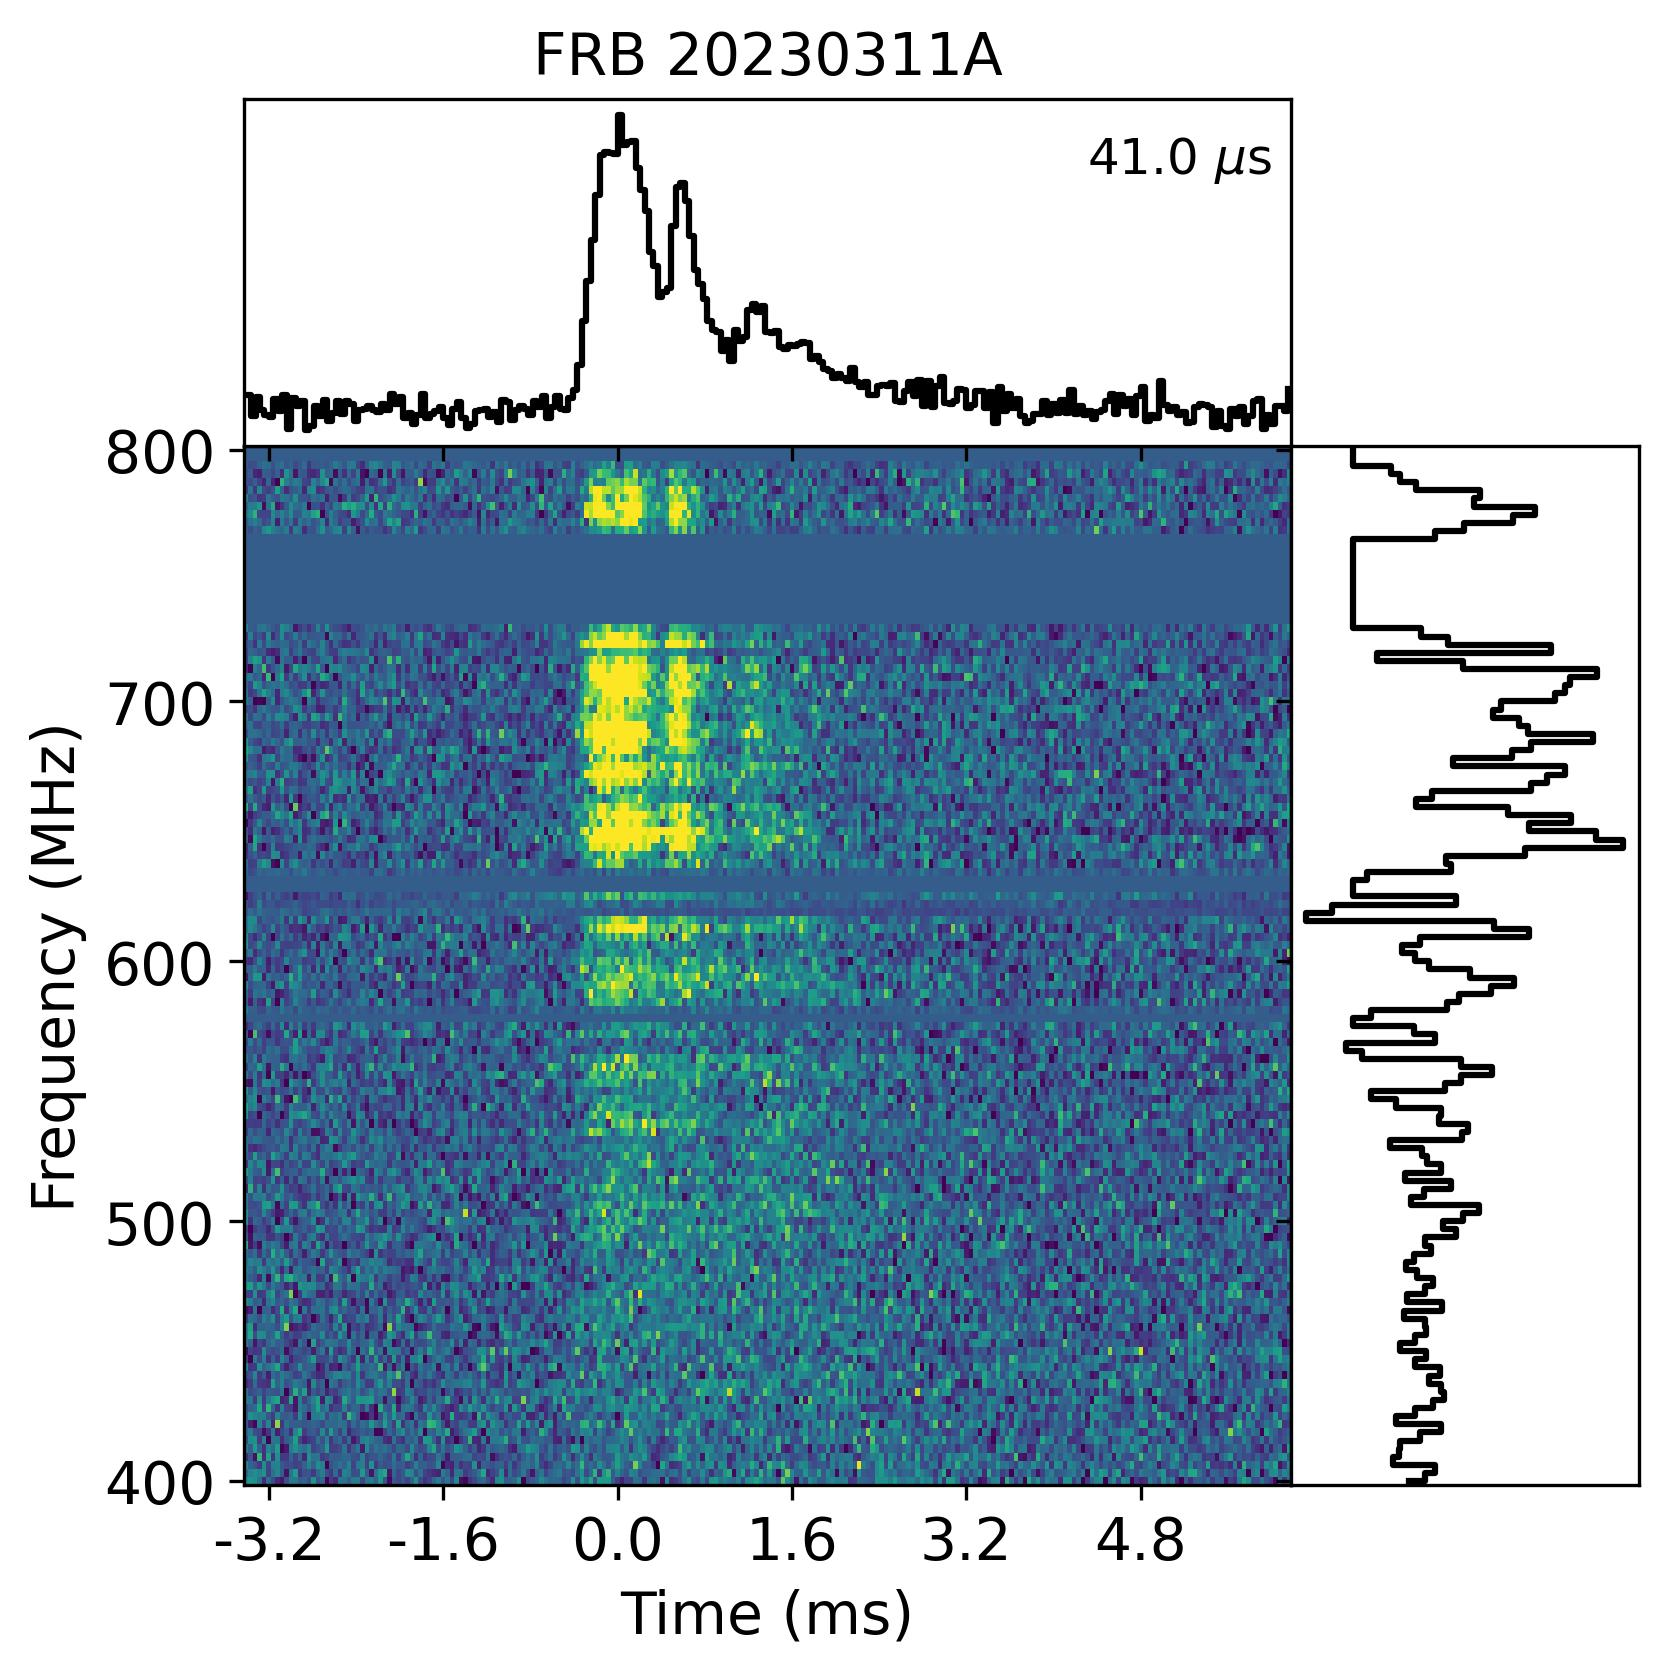
\includegraphics[width = 0.22\textwidth]{figures/FRB 20230311A_wfall.jpg} &
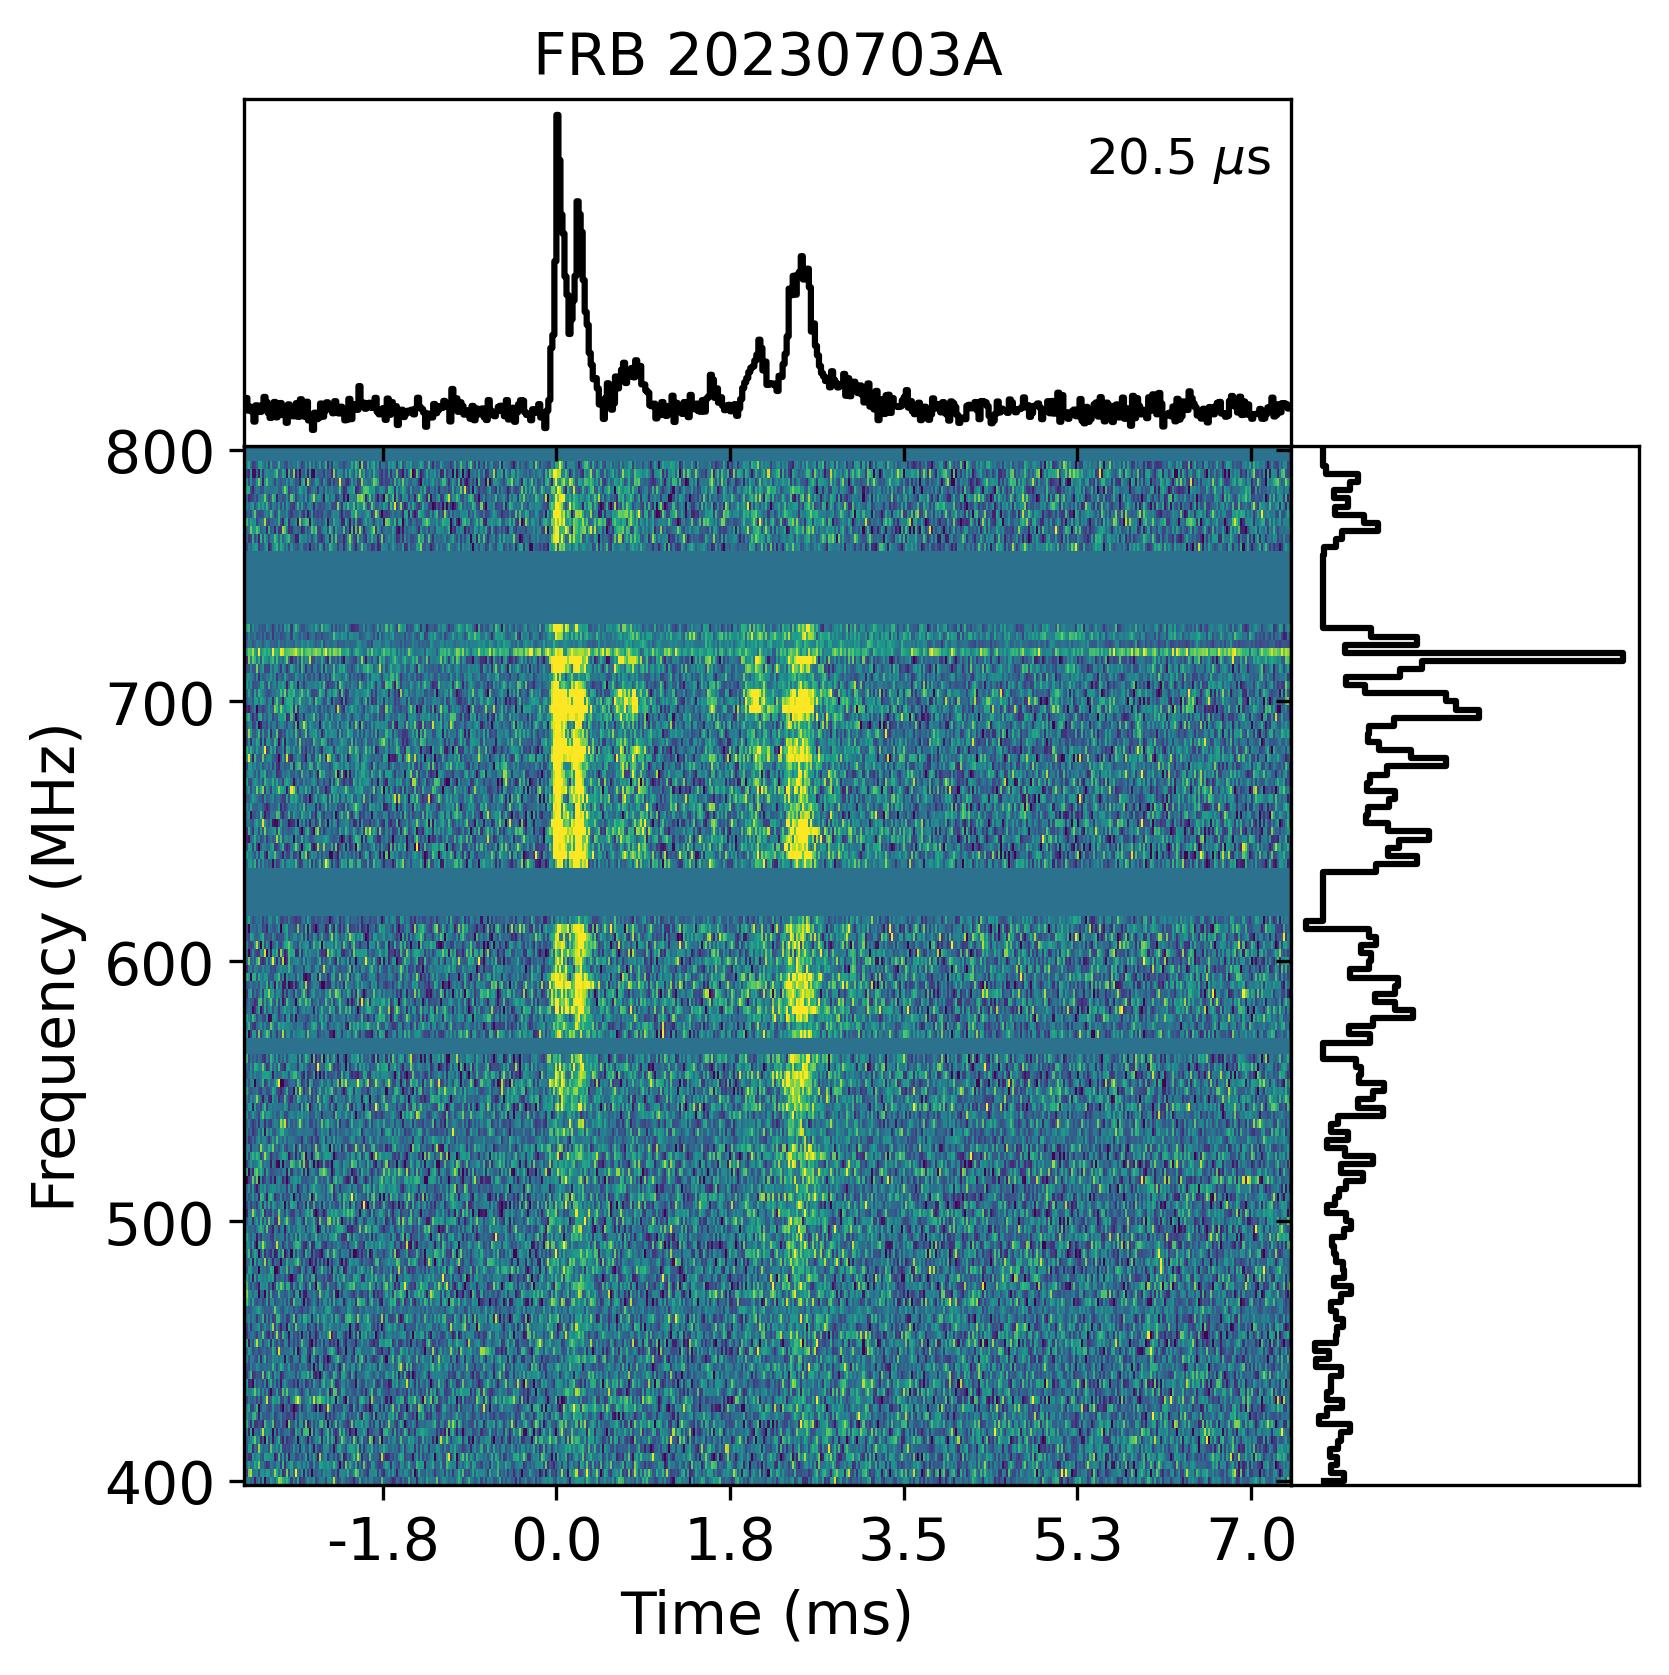
\includegraphics[width = 0.22\textwidth]{figures/FRB 20230703A_wfall.jpg} &
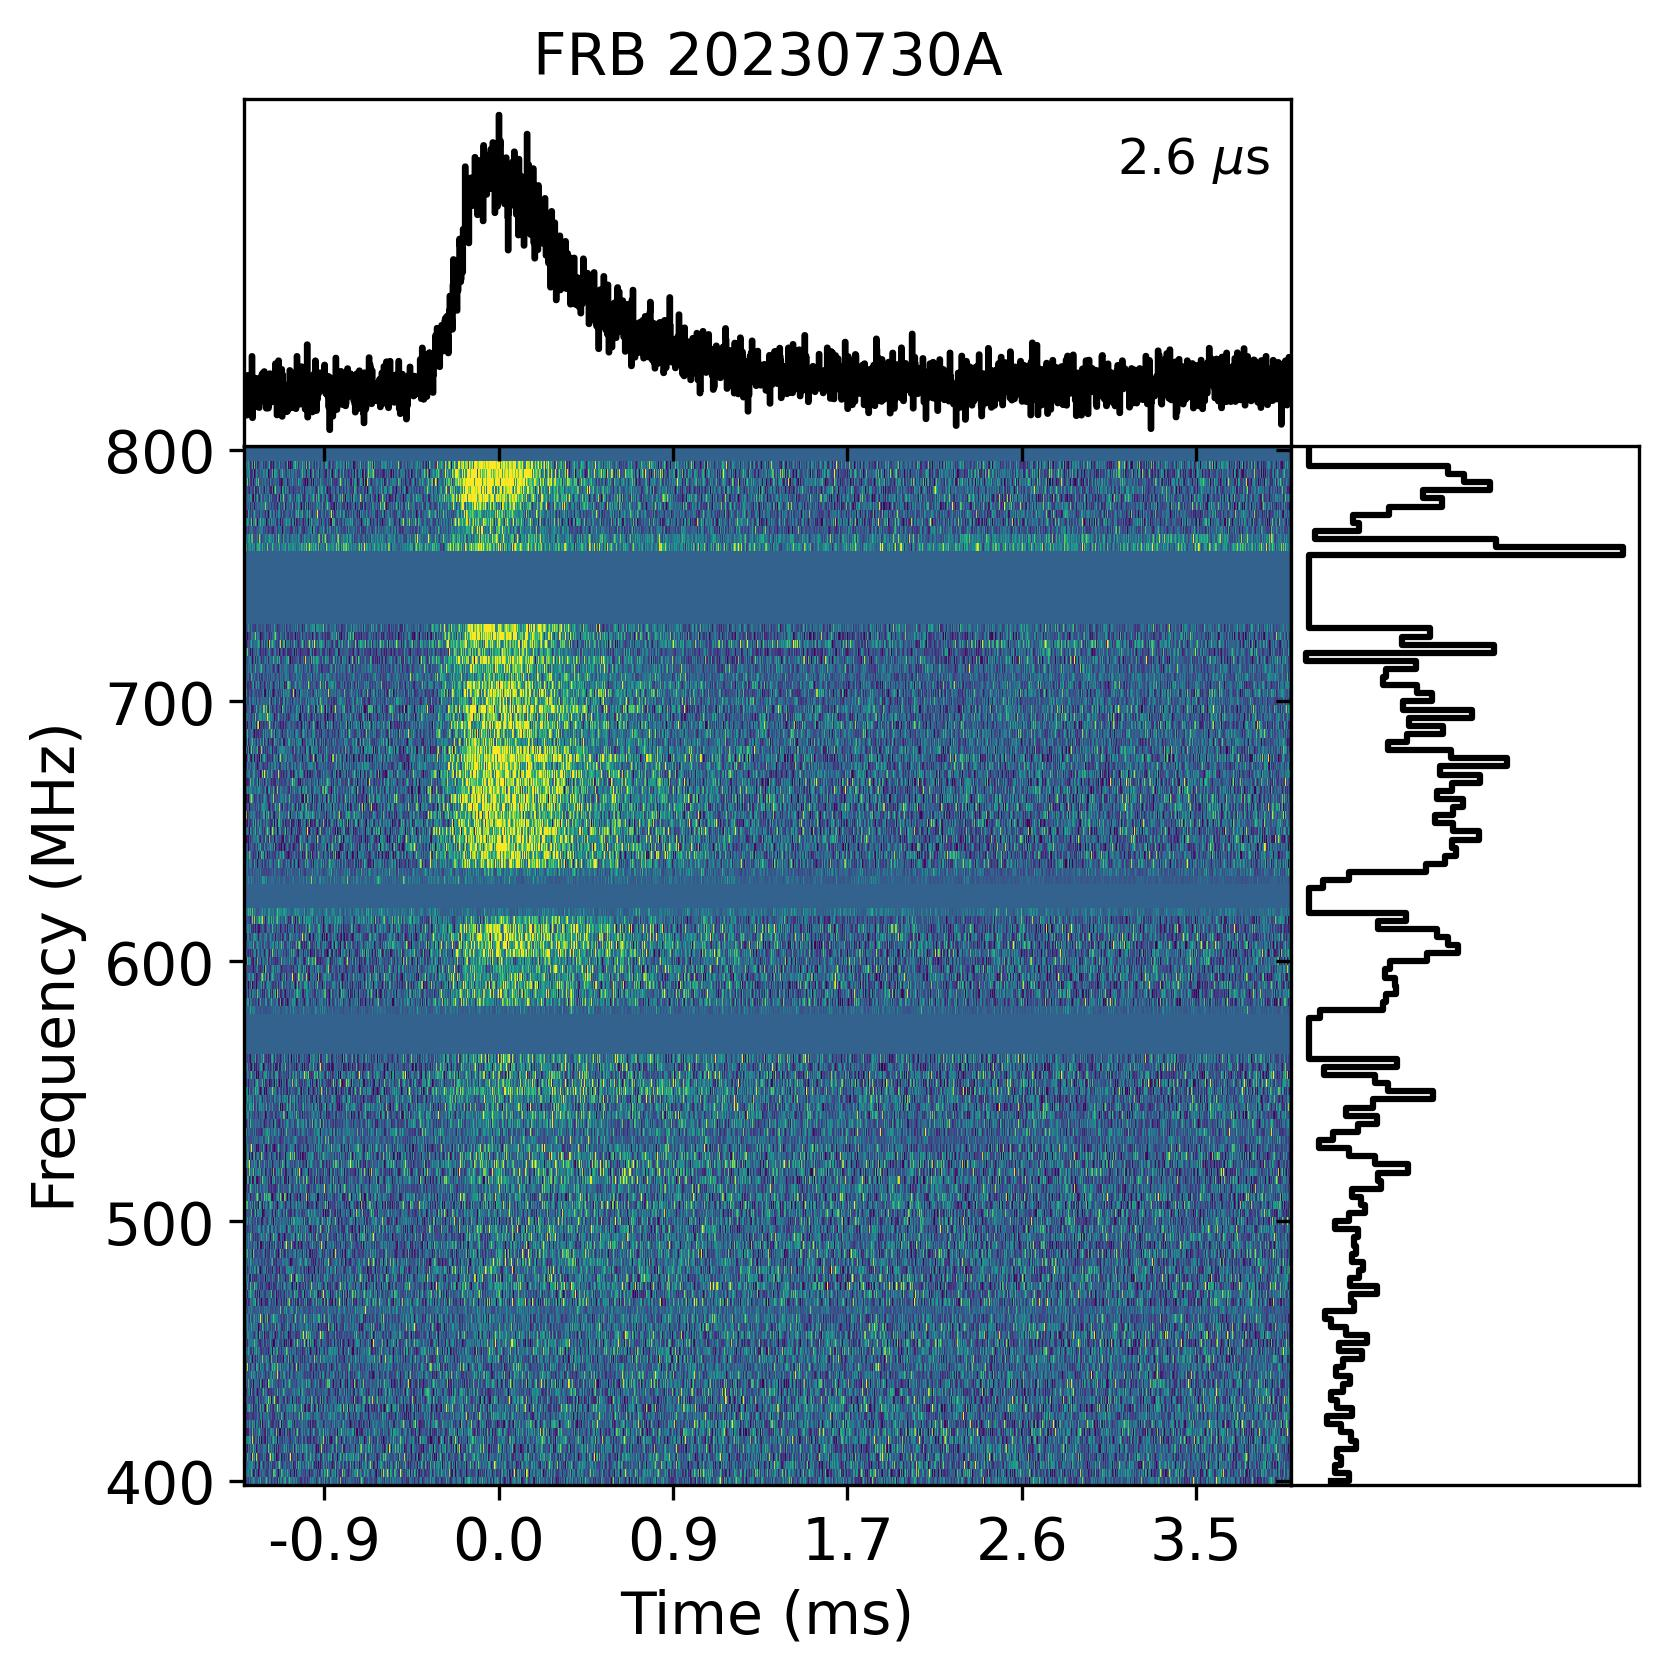
\includegraphics[width = 0.22\textwidth]{figures/FRB 20230730A_wfall.jpg} \\
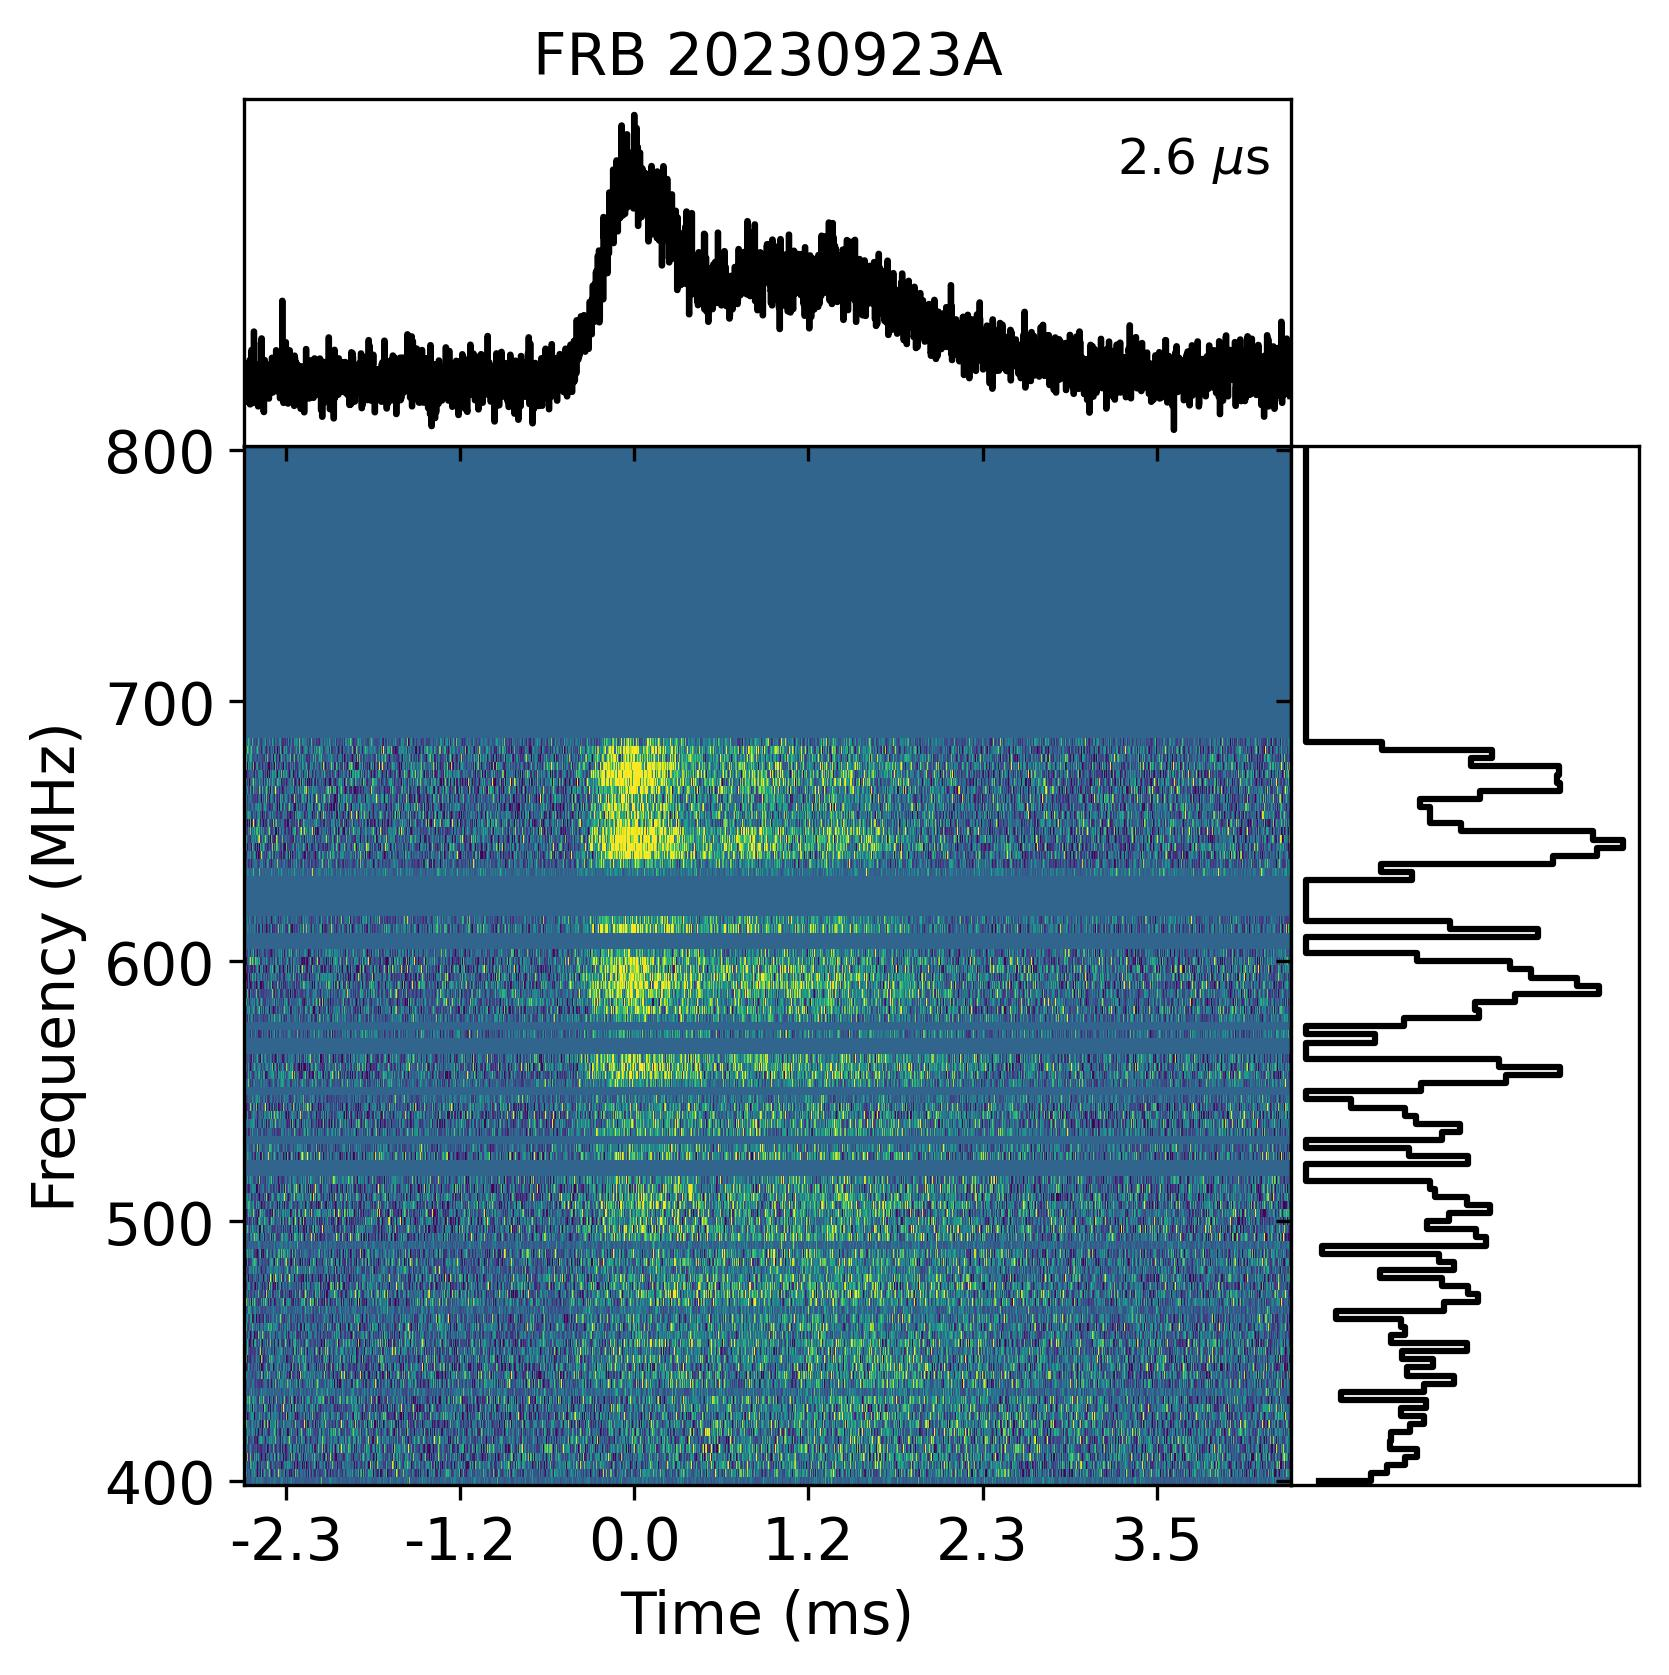
\includegraphics[width = 0.22\textwidth]{figures/FRB 20230923A_wfall.jpg} &
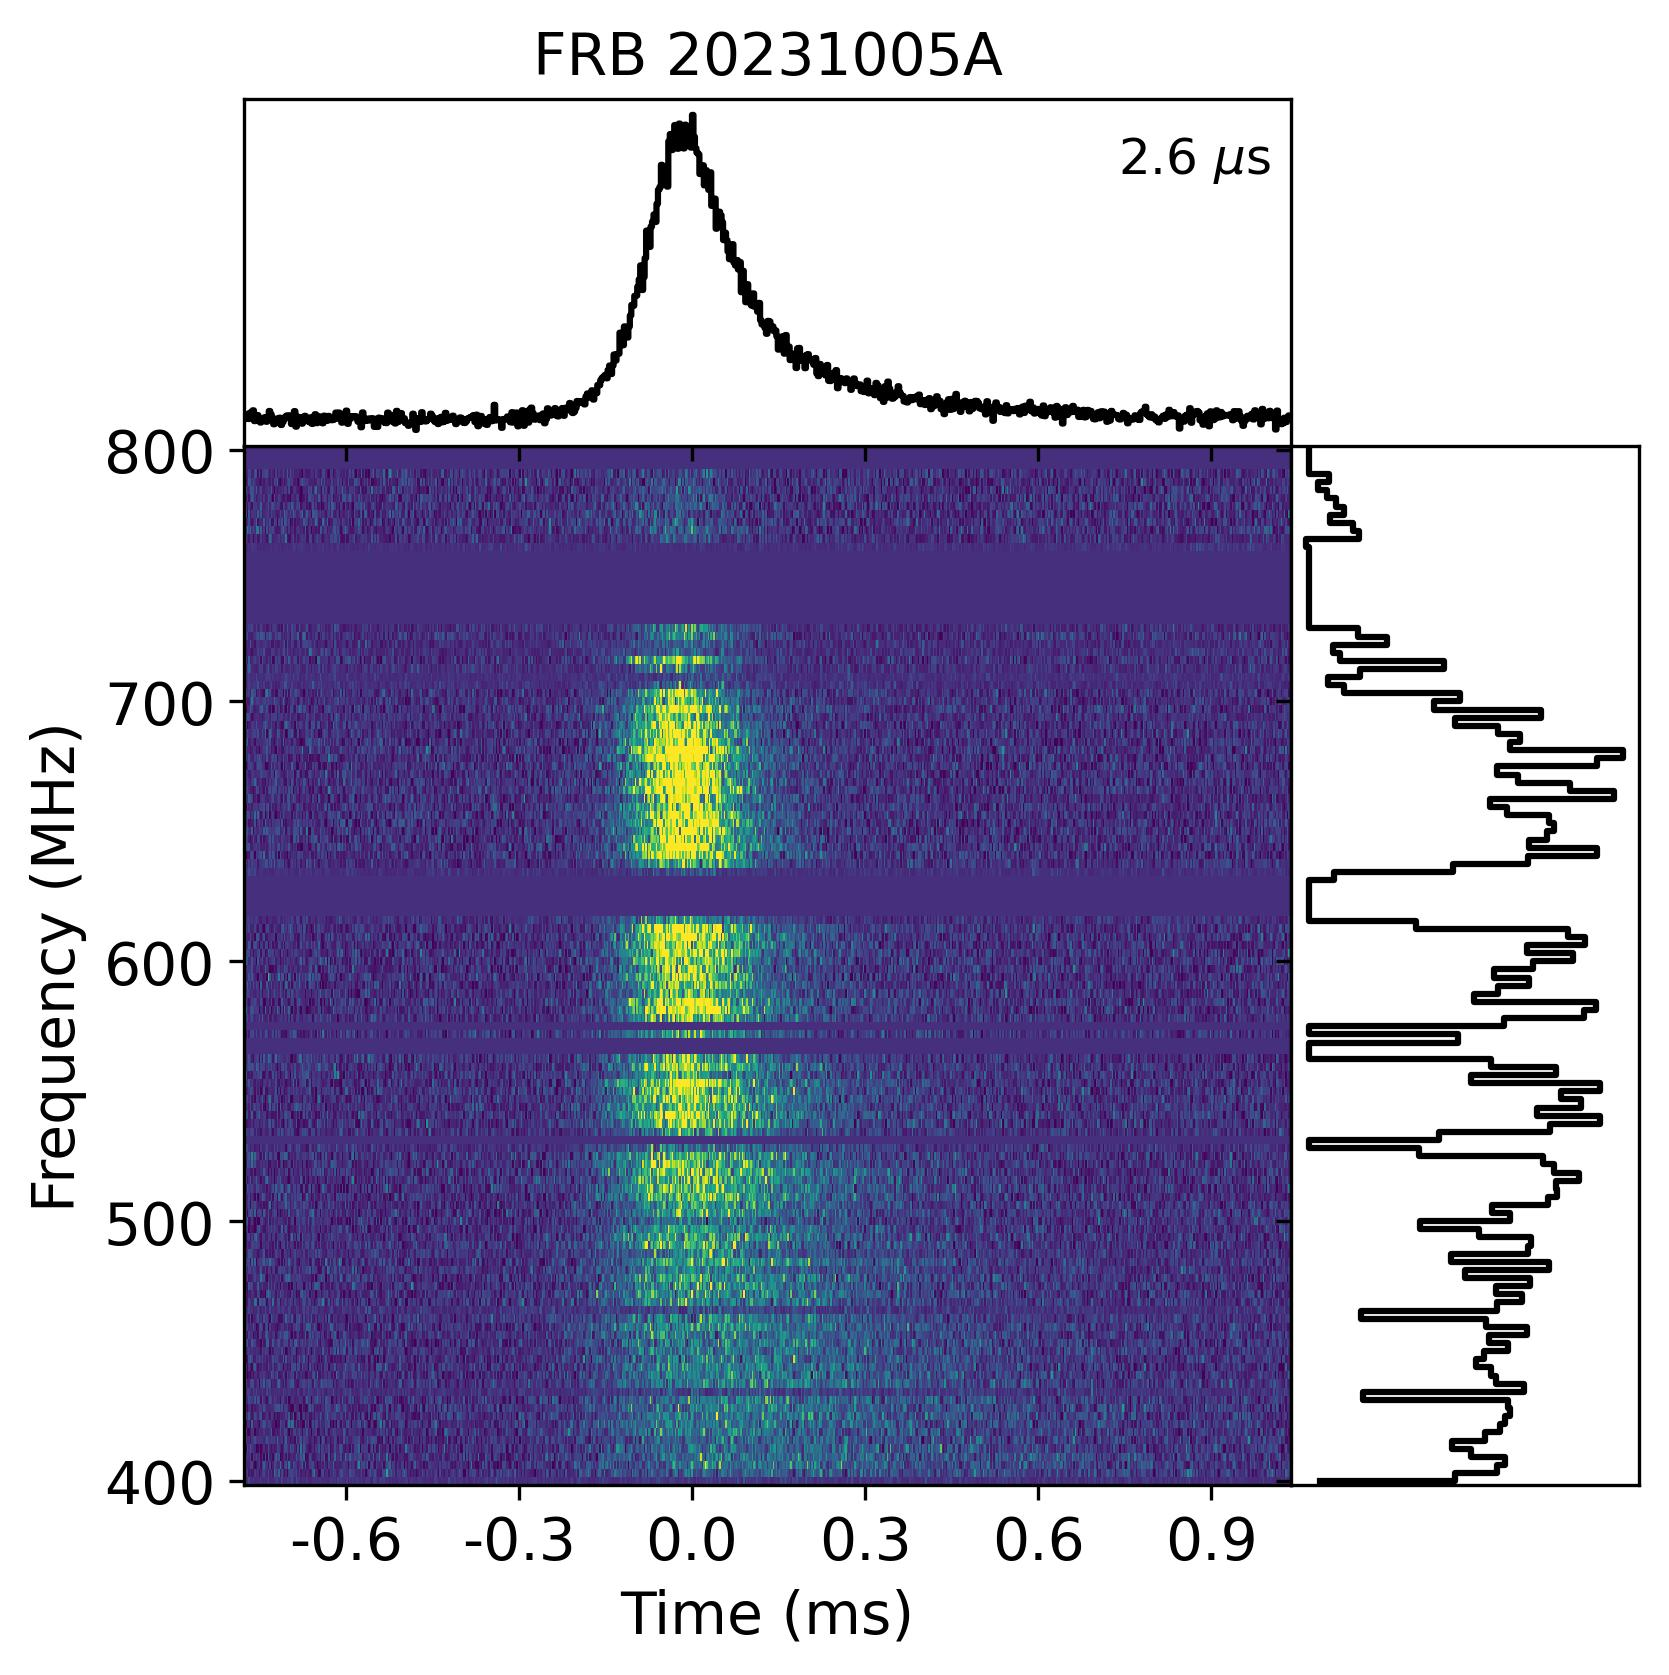
\includegraphics[width = 0.22\textwidth]{figures/FRB 20231005A_wfall.jpg} &
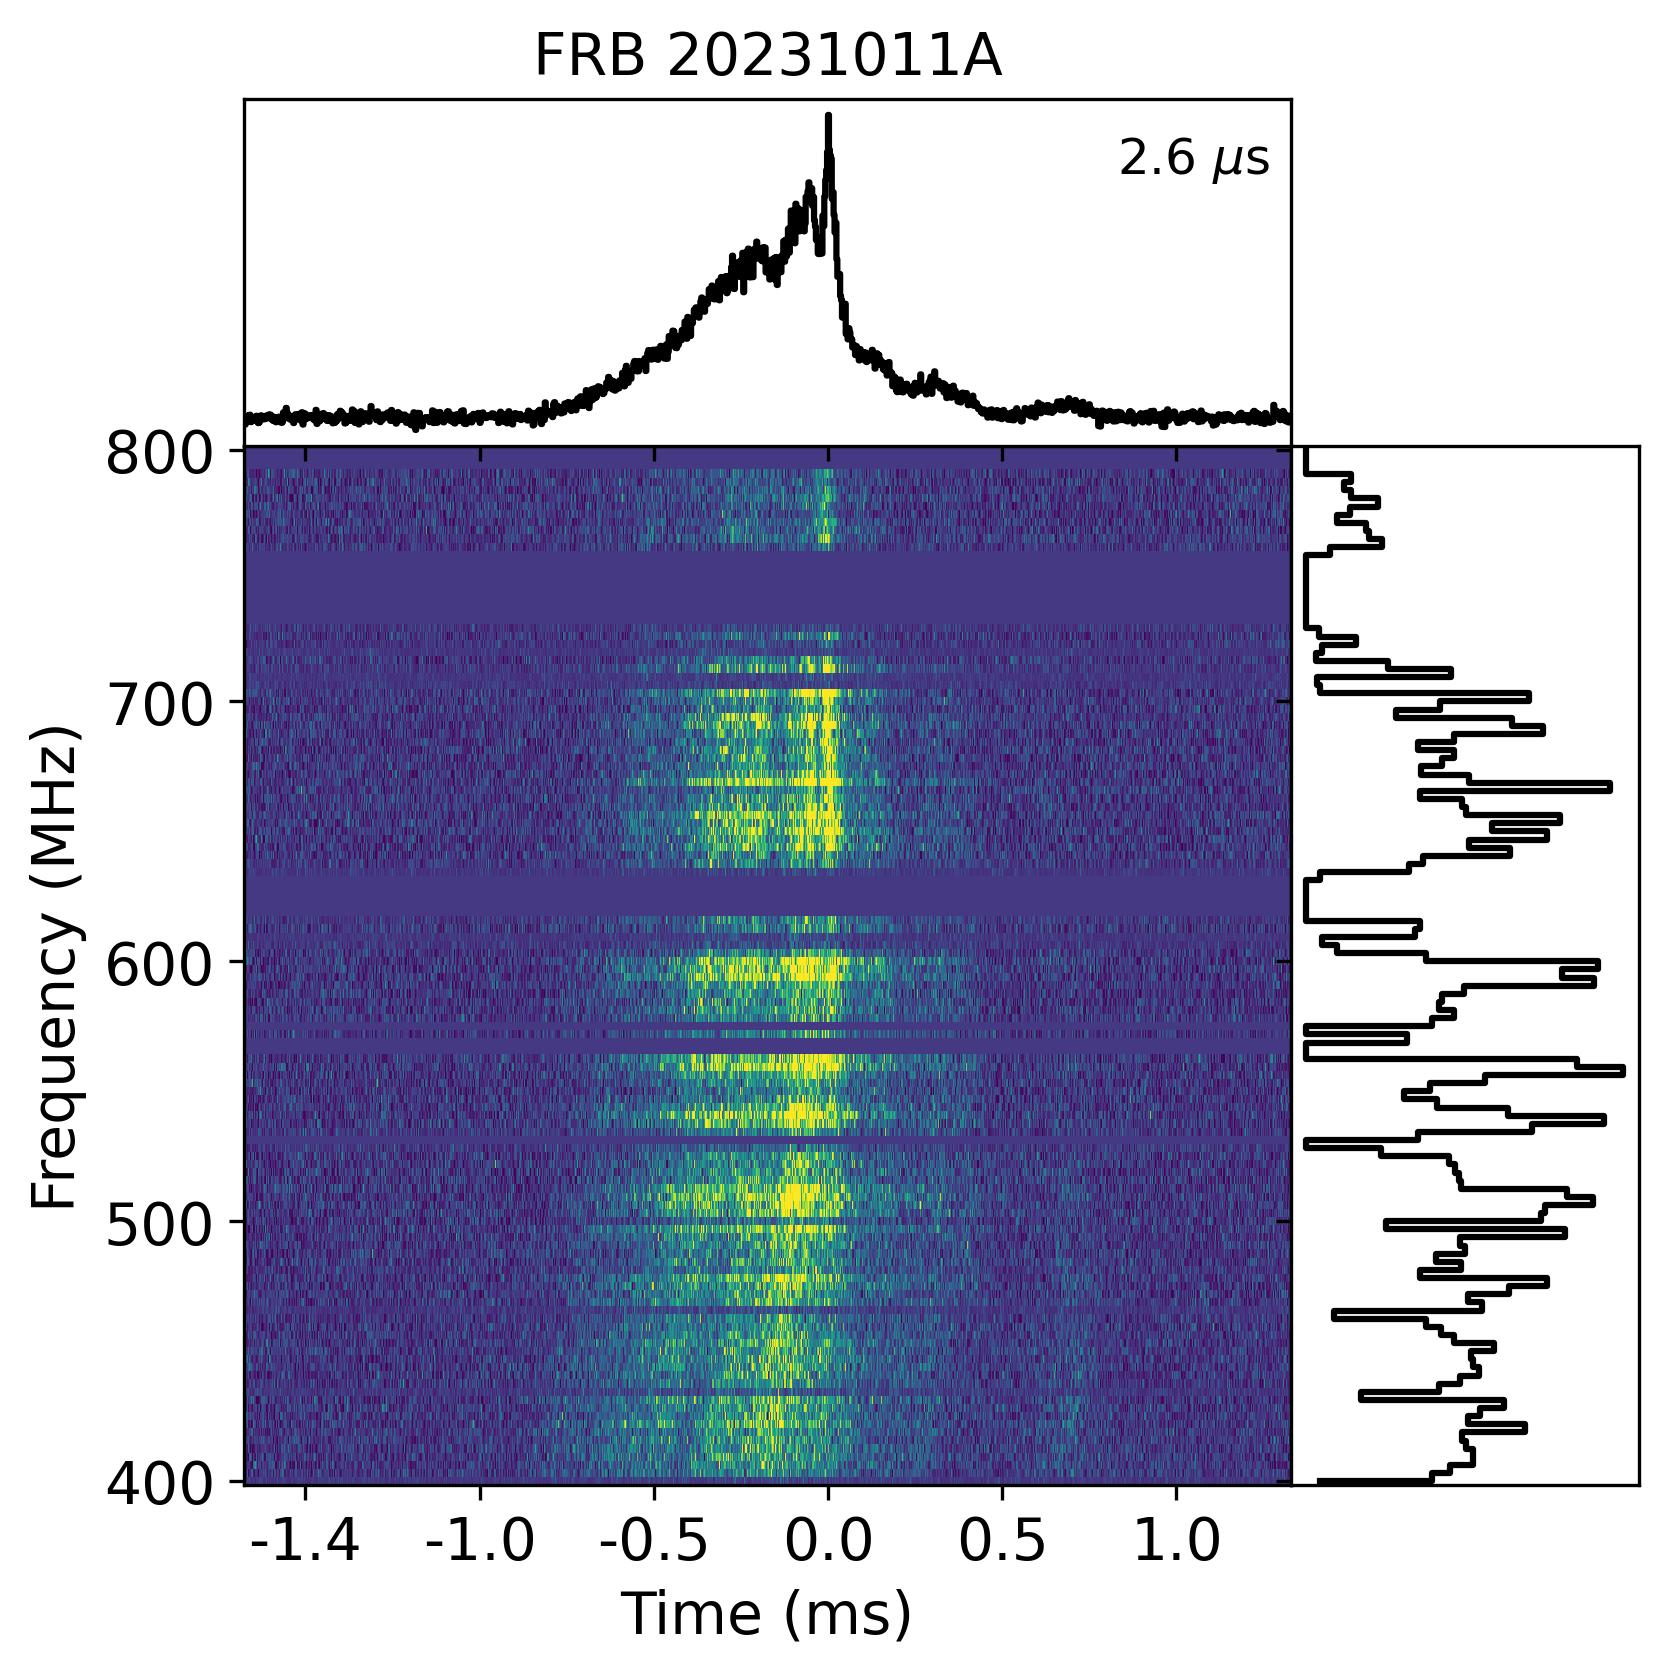
\includegraphics[width = 0.22\textwidth]{figures/FRB 20231011A_wfall.jpg} &
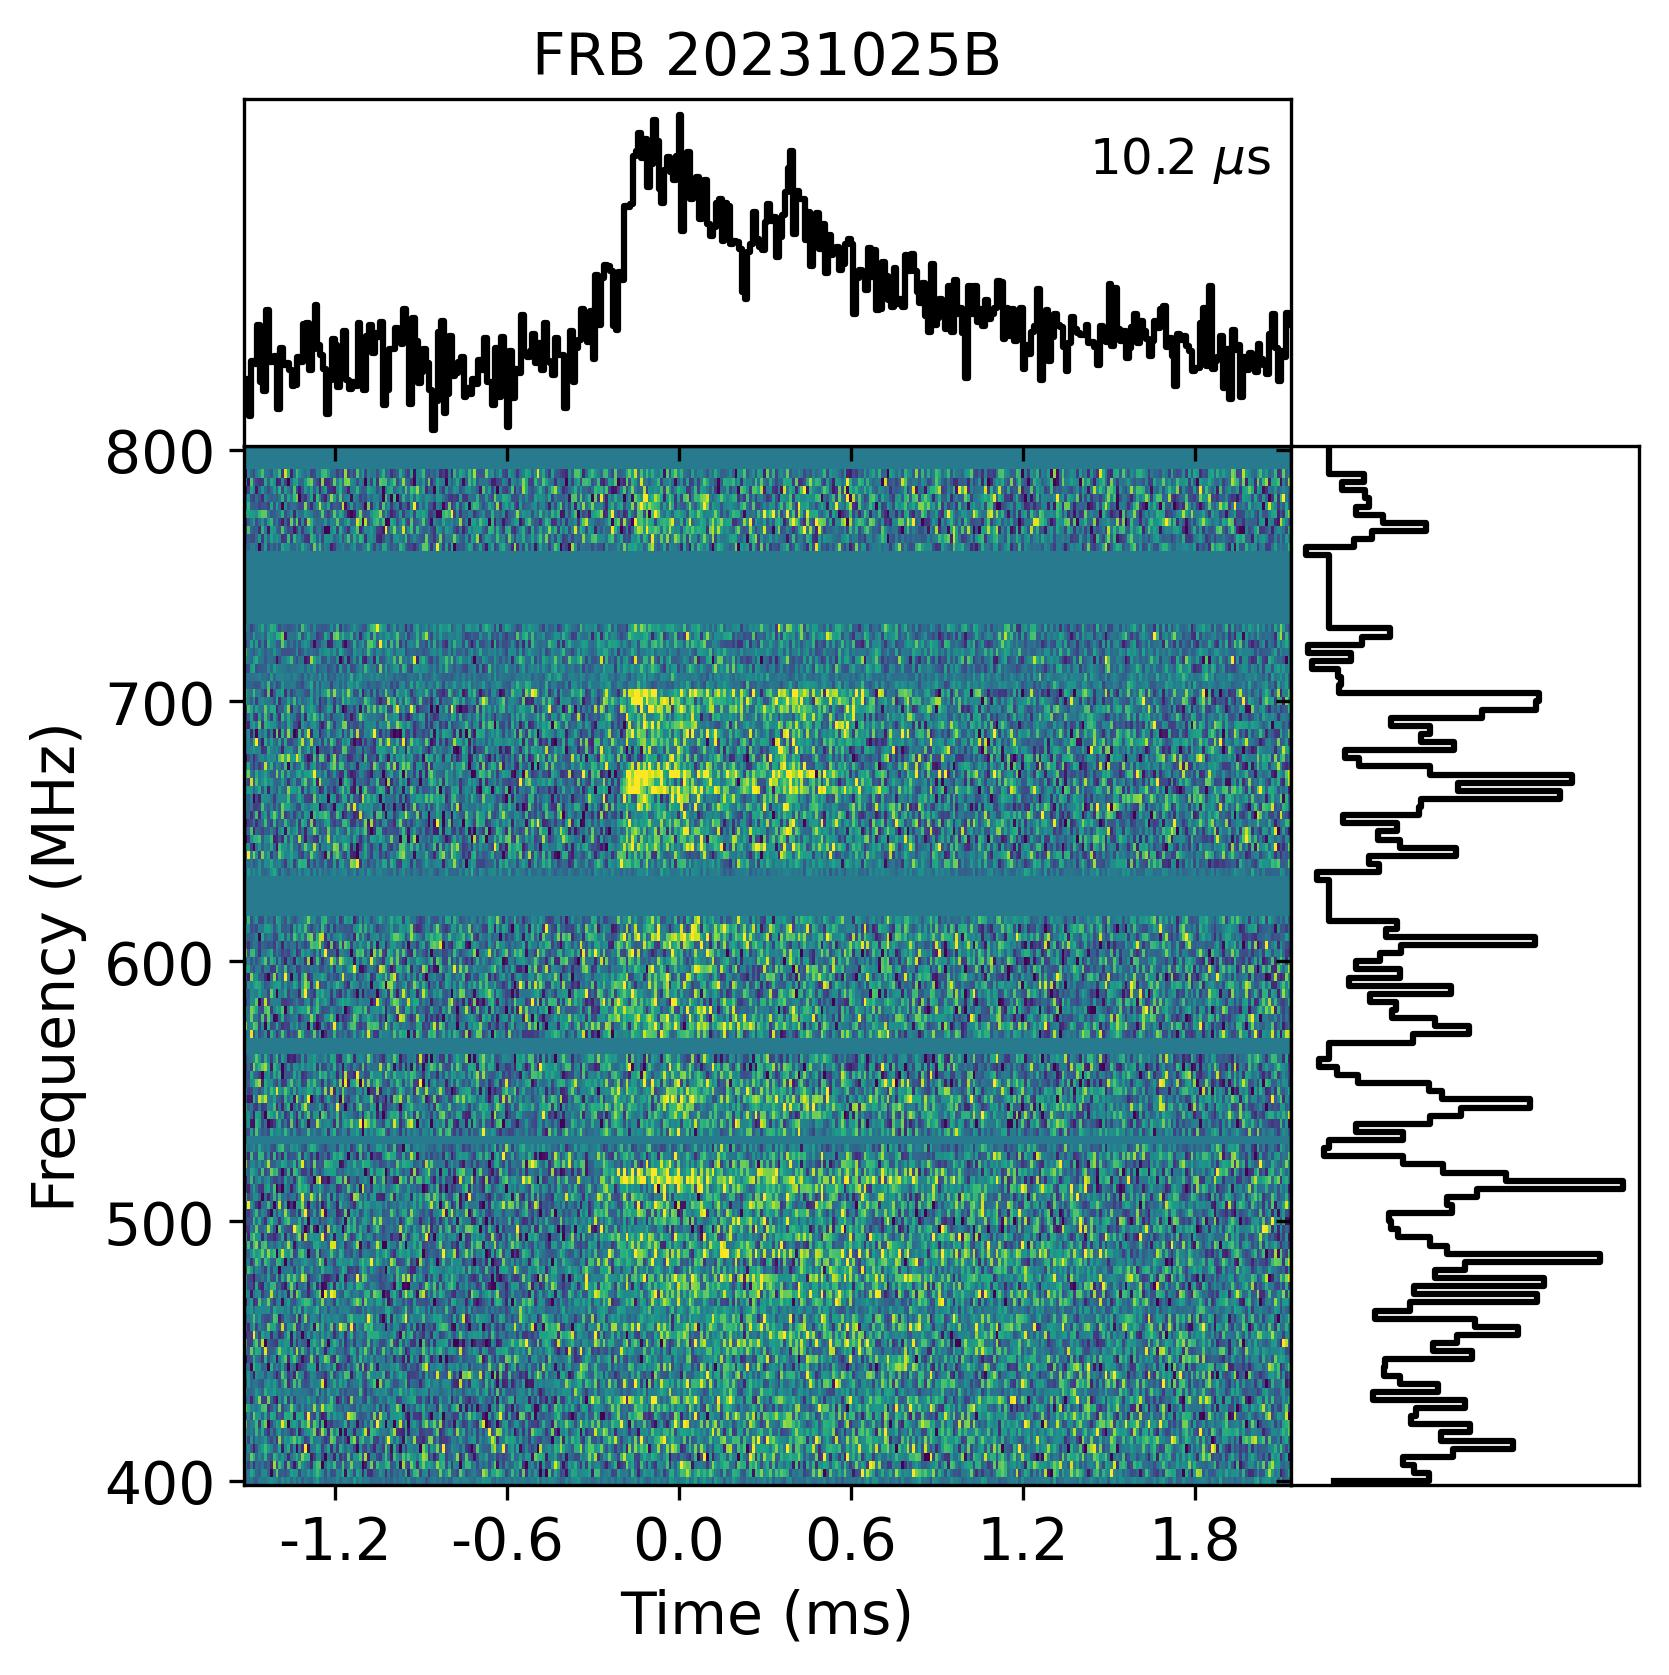
\includegraphics[width = 0.22\textwidth]{figures/FRB 20231025B_wfall.jpg}
\\
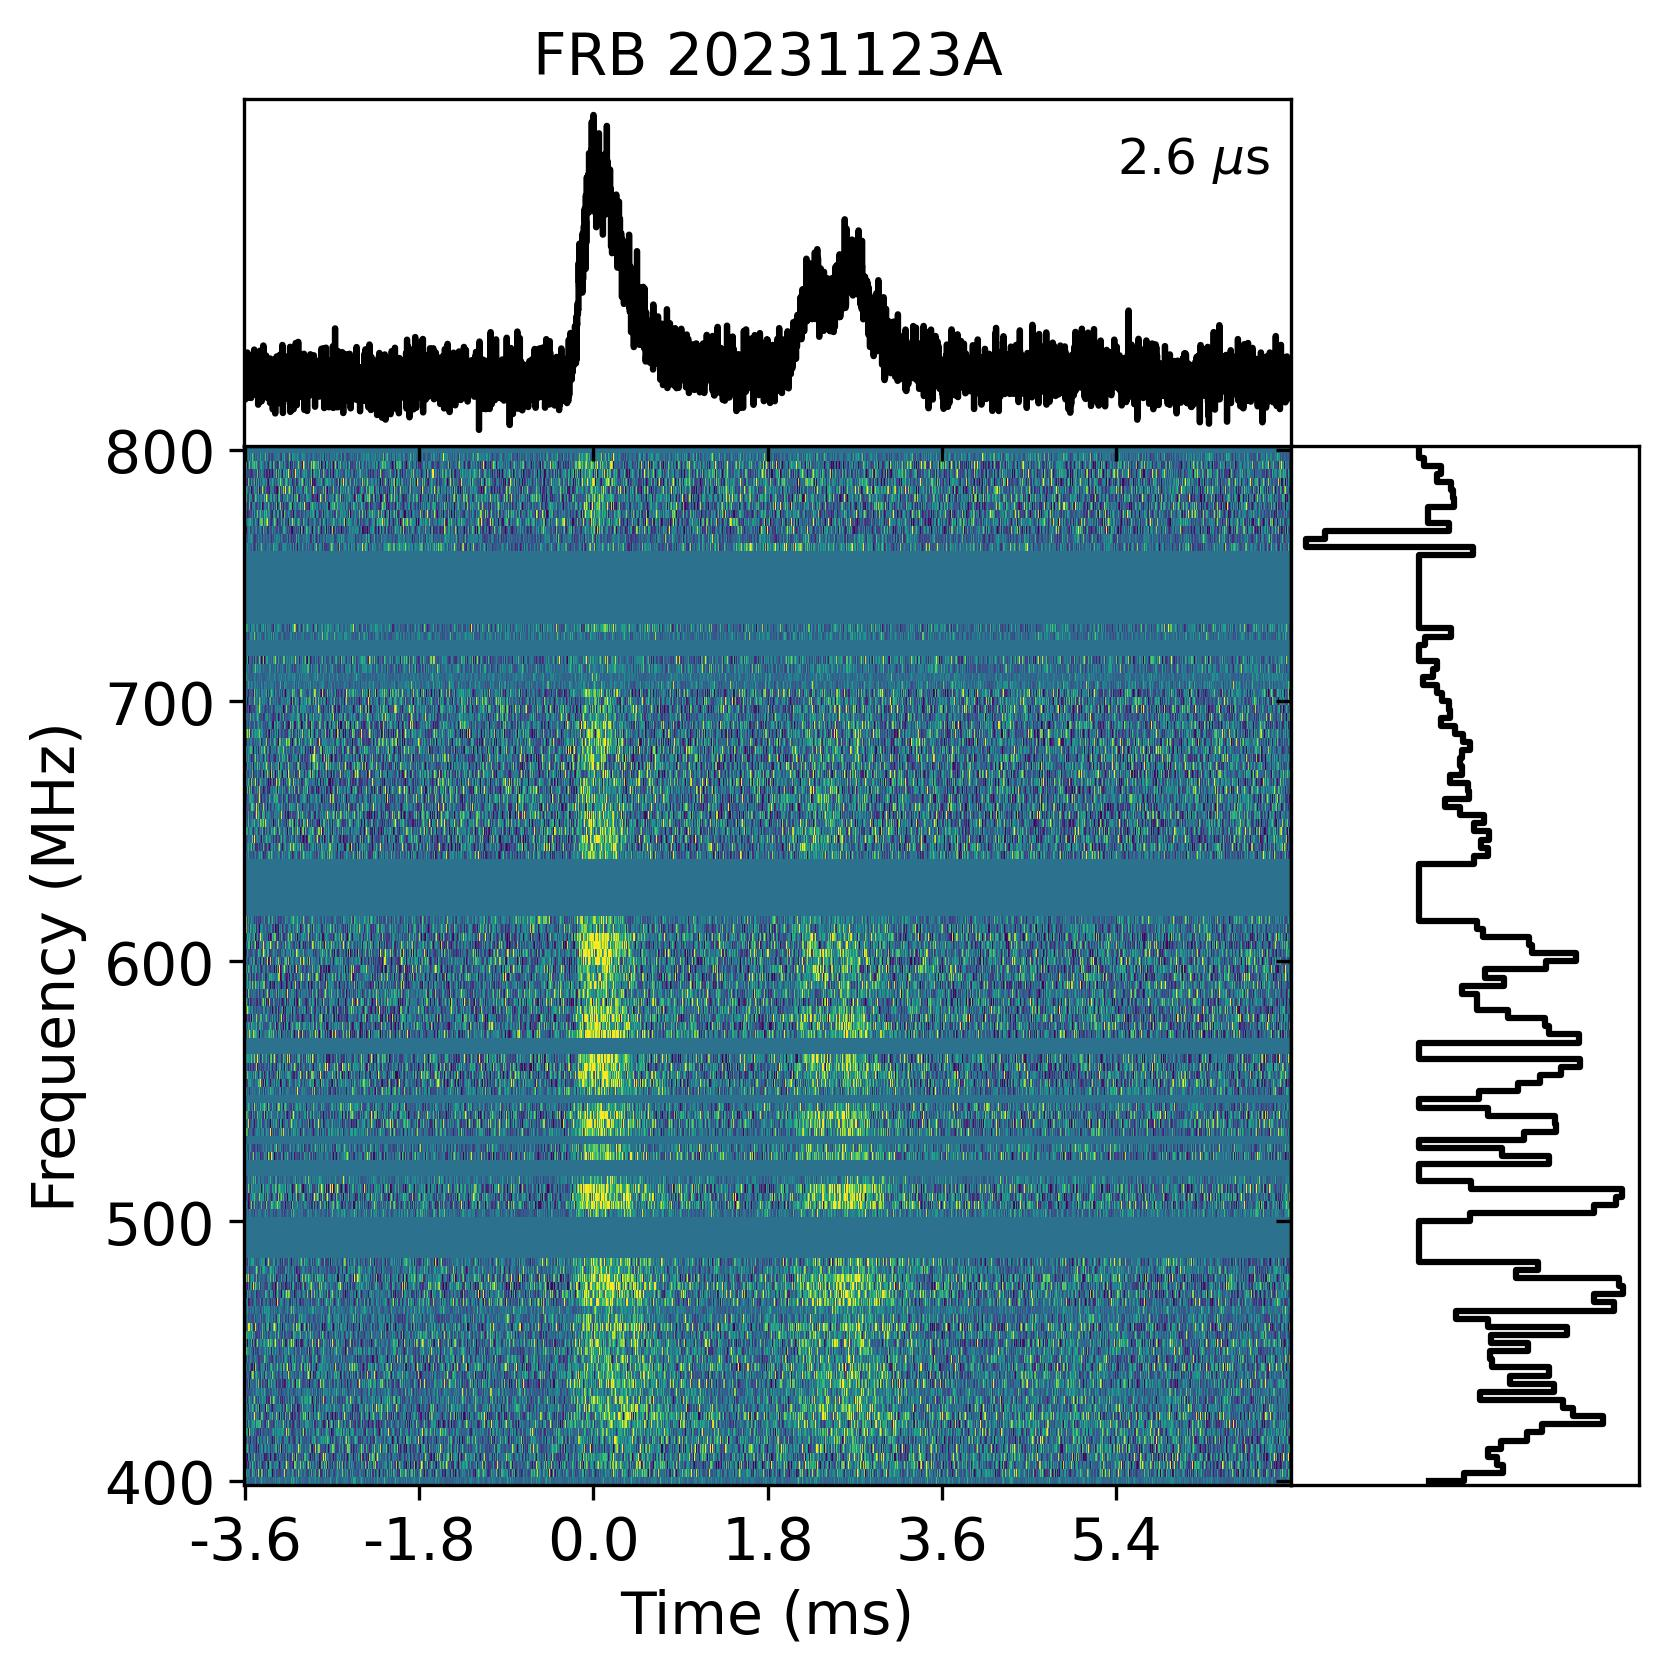
\includegraphics[width = 0.22\textwidth]{figures/FRB 20231123A_wfall.jpg}
&
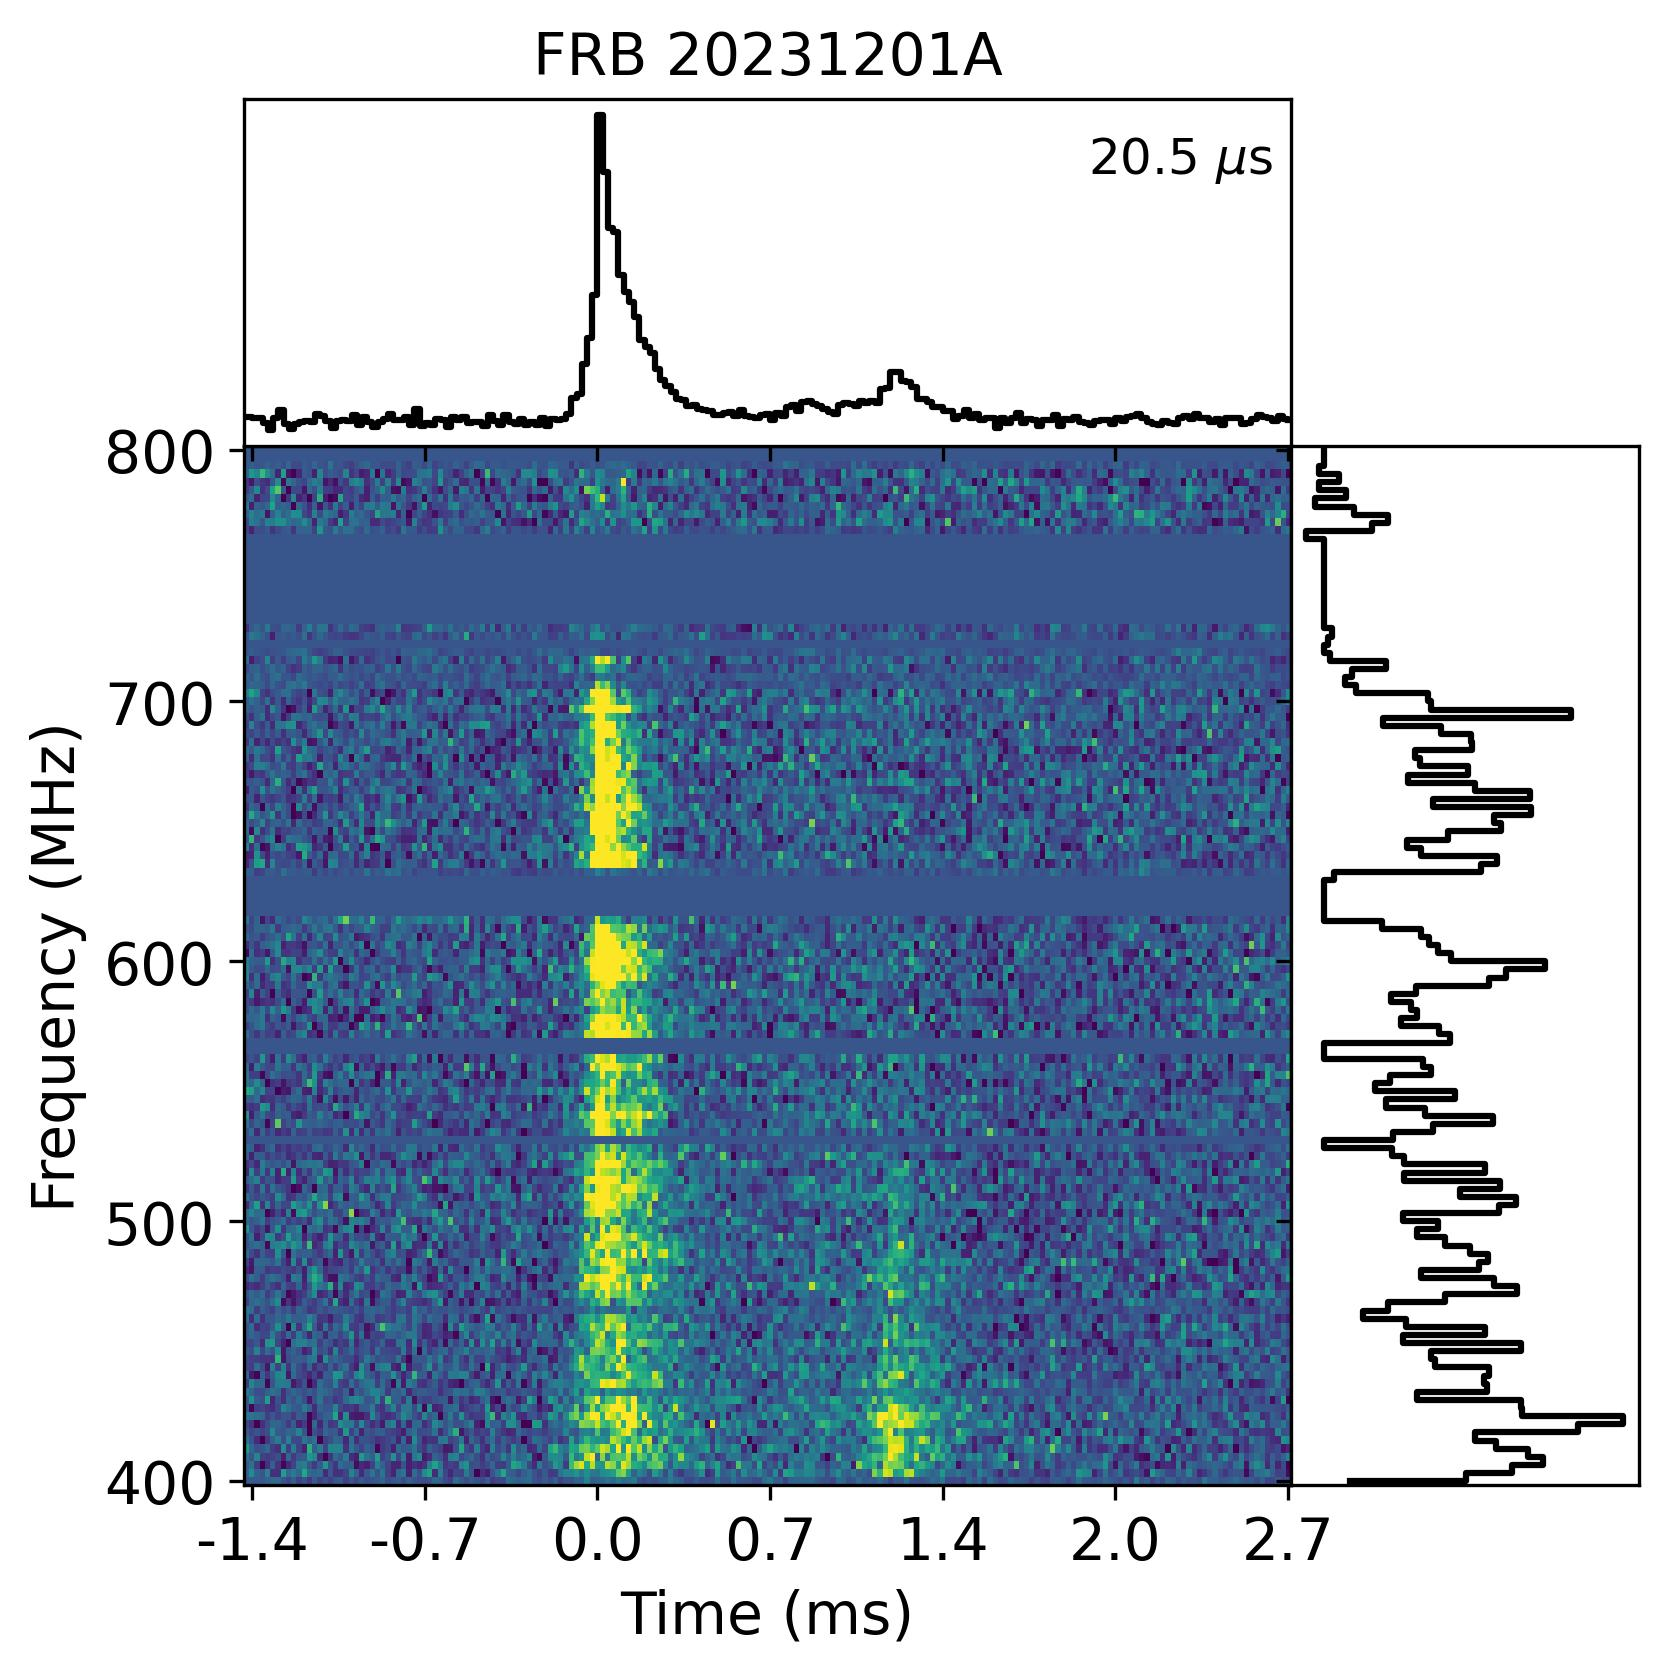
\includegraphics[width = 0.22\textwidth]{figures/FRB 20231201A_wfall.jpg}
&
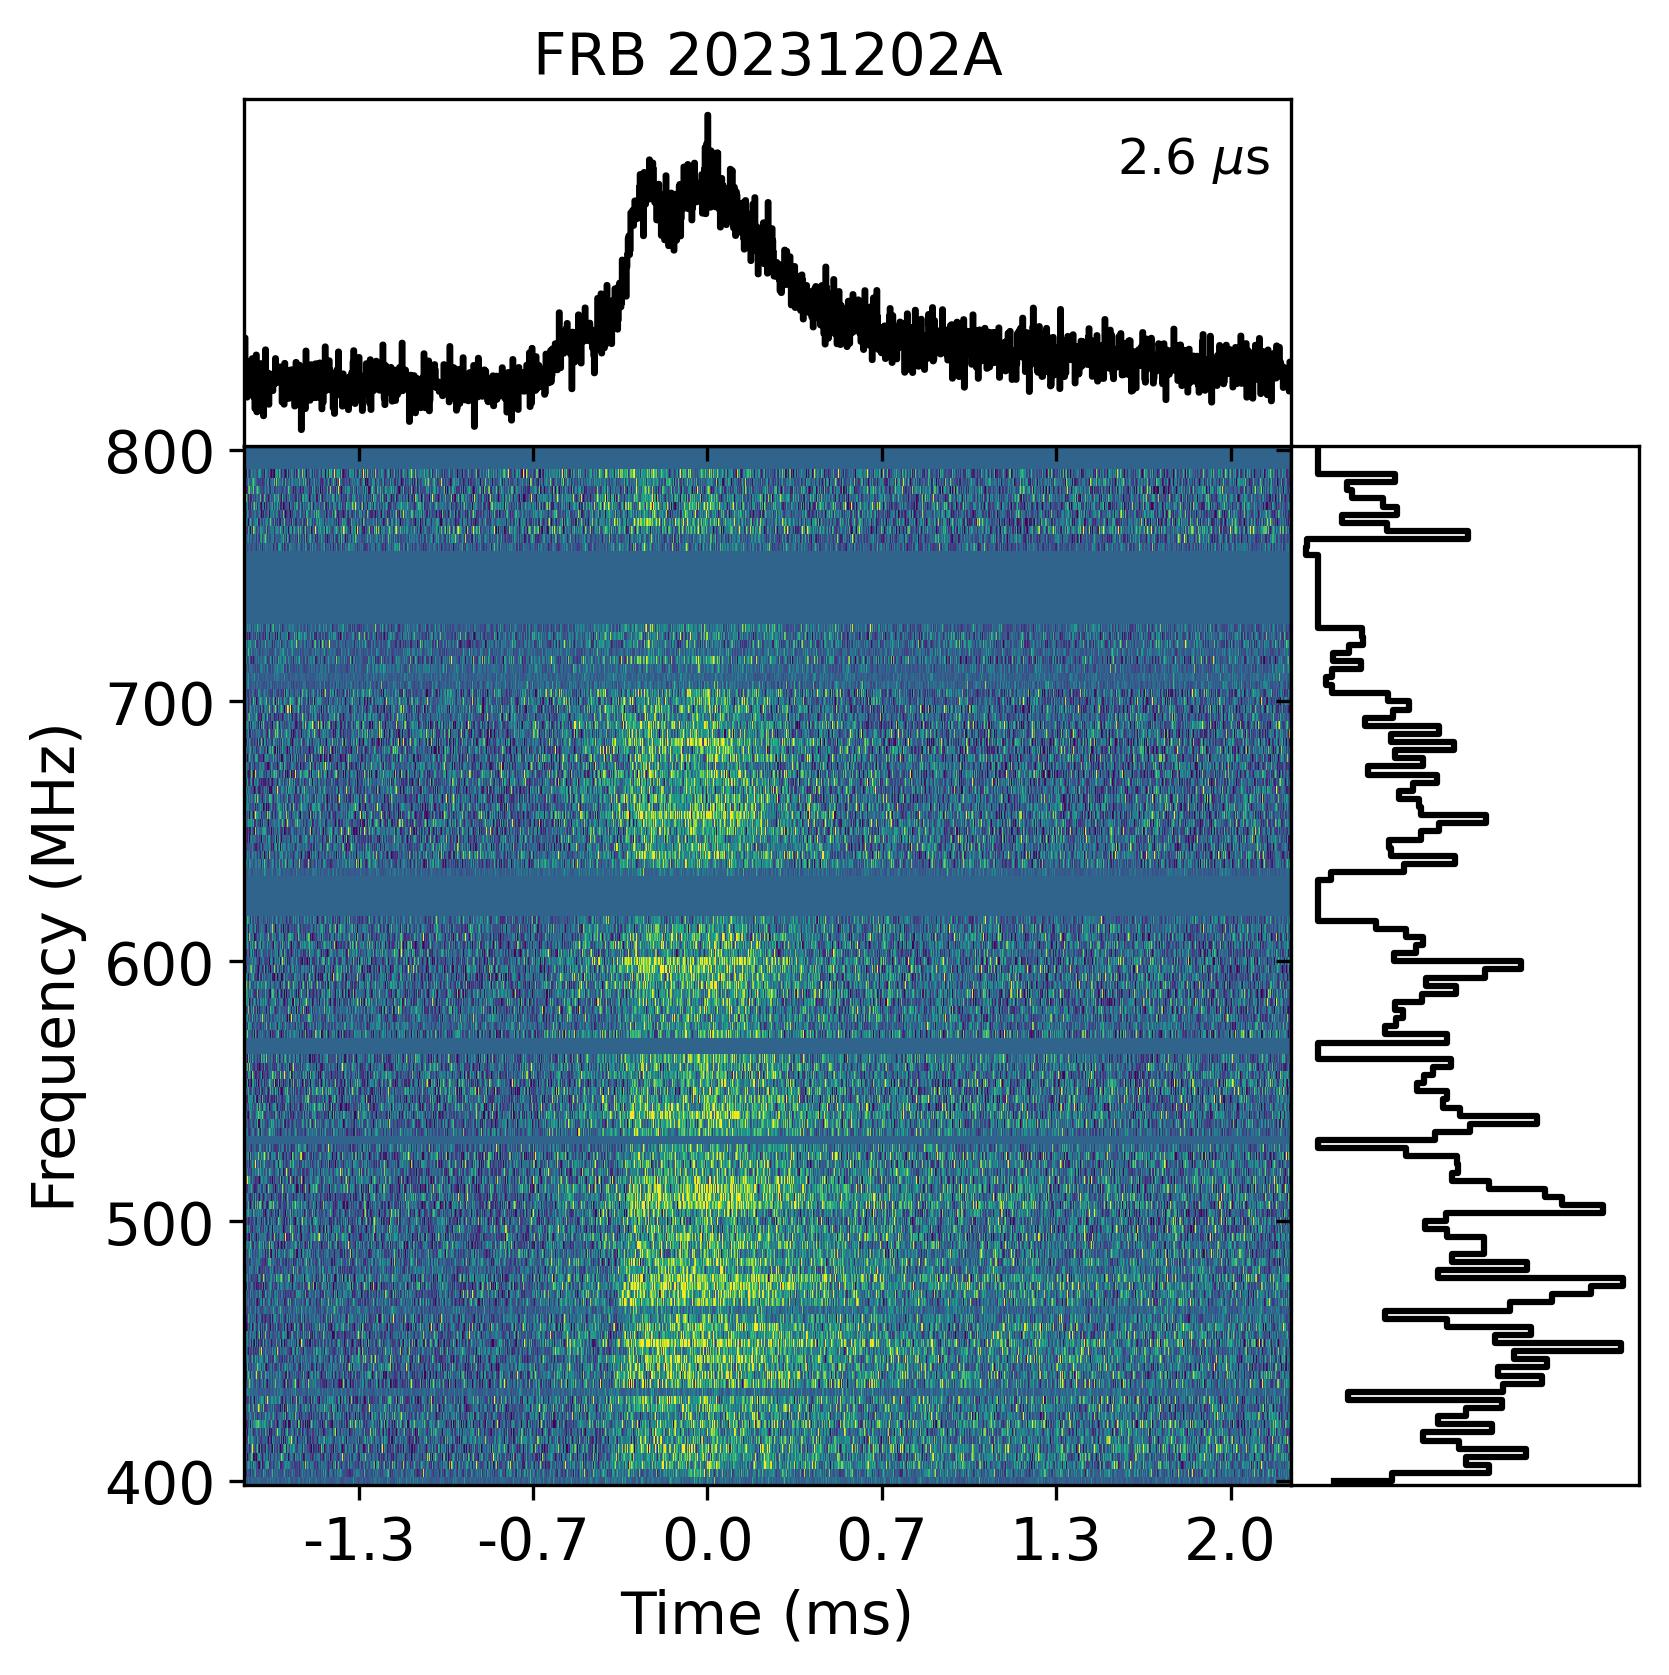
\includegraphics[width = 0.22\textwidth]{figures/FRB 20231202A_wfall.jpg} &
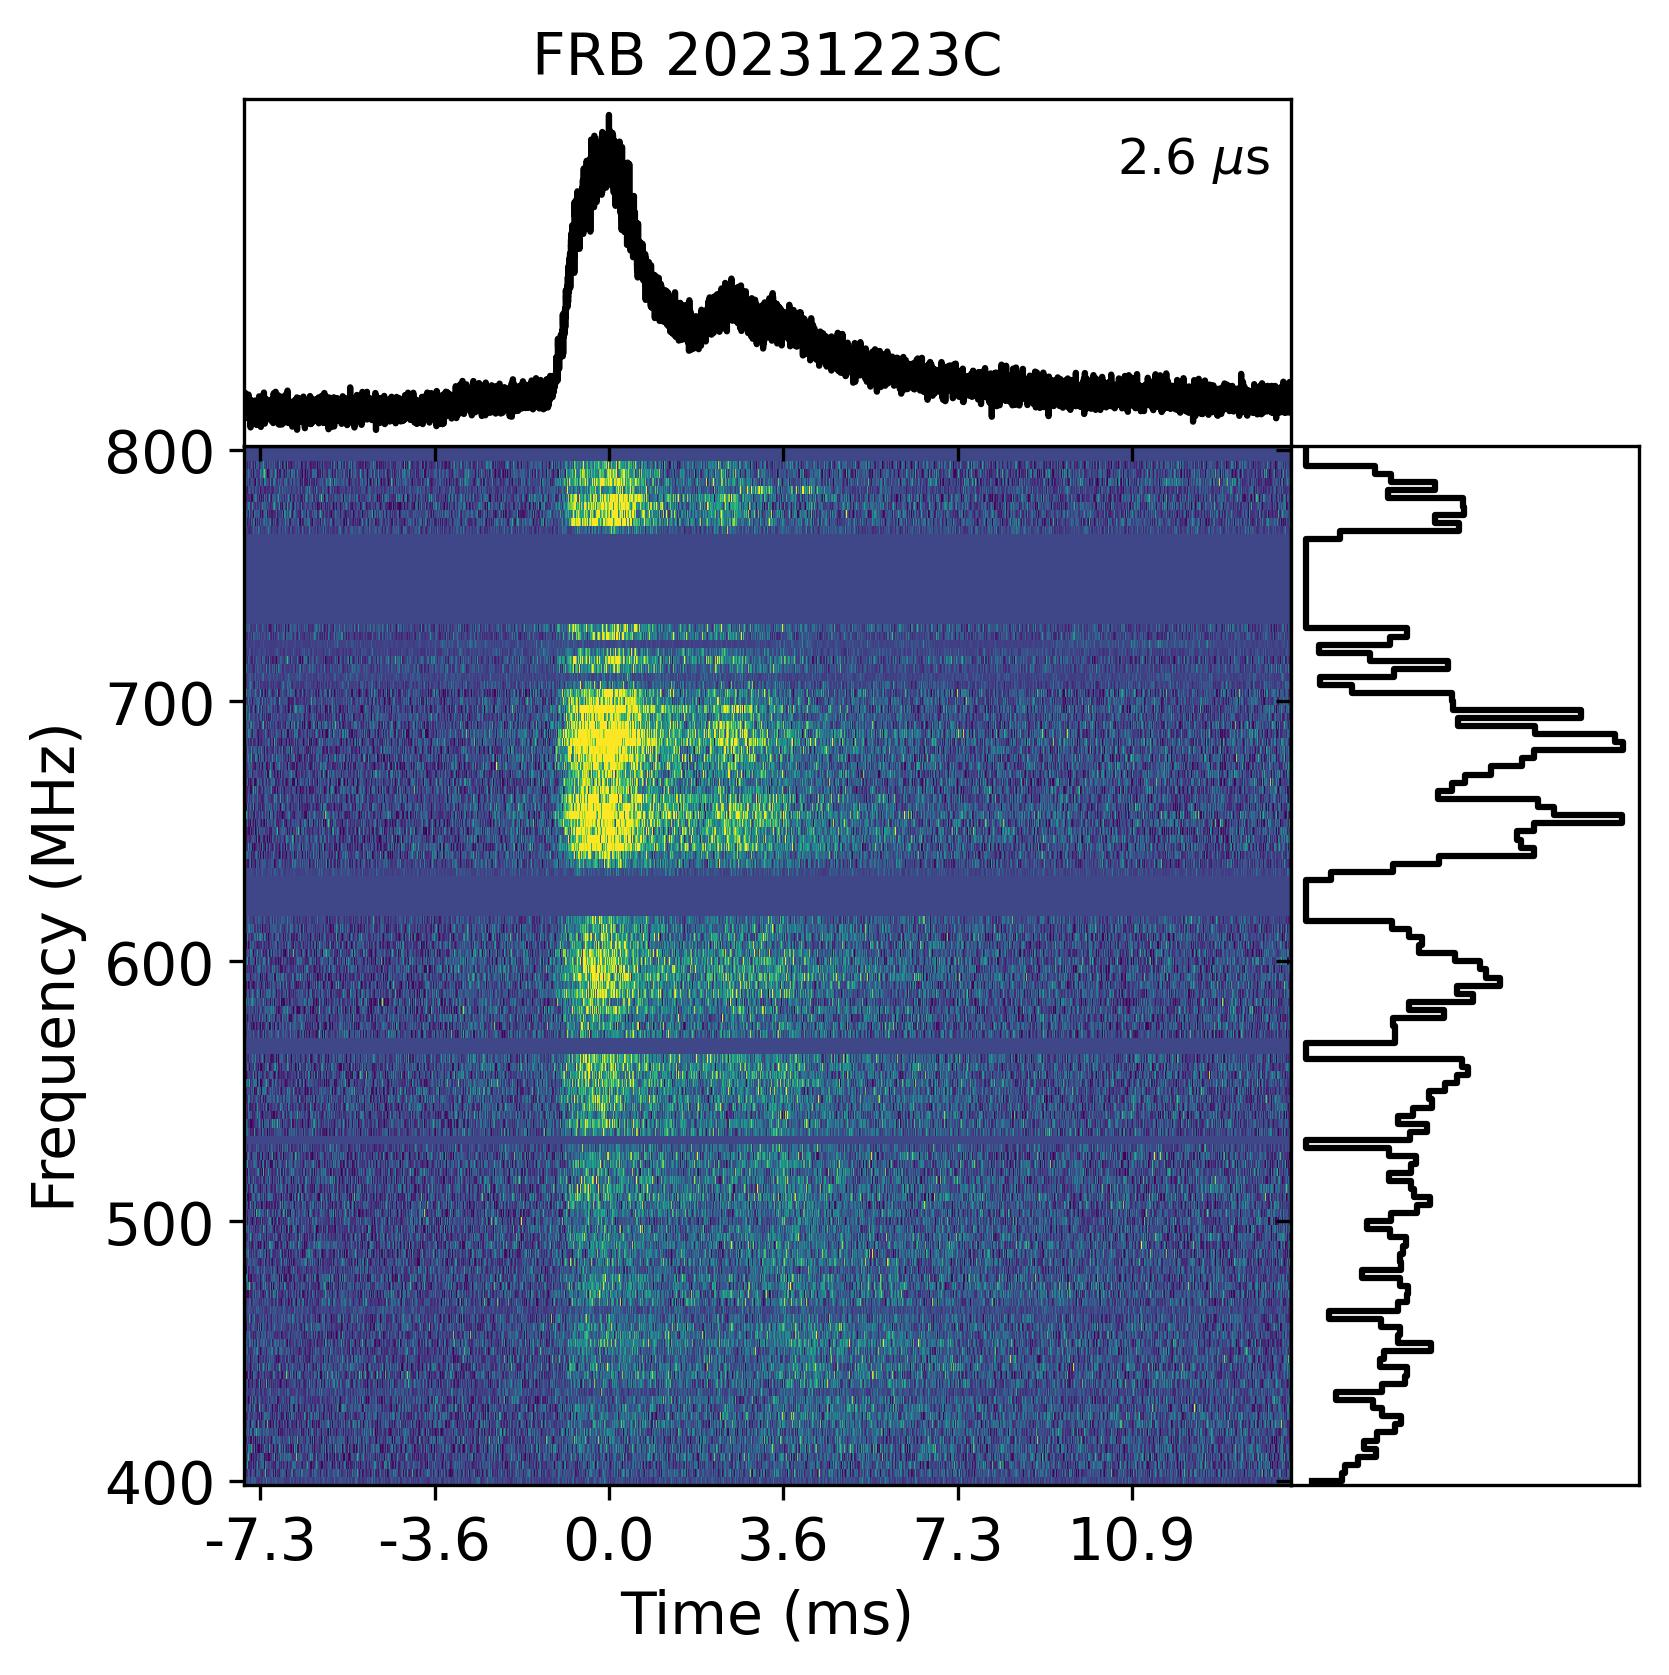
\includegraphics[width = 0.22\textwidth]{figures/FRB 20231223C_wfall.jpg} \\

%\subfloat[caption]{\includegraphics[width = 1.5in]{something}}\\
%\subfloat[caption]{\includegraphics[width = 1.5in]{something}} &
%\subfloat[caption]{\includegraphics[width = 1.5in]{something}} &
%\subfloat[caption]{\includegraphics[width = 1.5in]{something}} &
%\subfloat[caption]{\includegraphics[width = 1.5in]{something}}
\end{tabular}
\caption{Waterfall plots of the bursts.}
\end{figure*}
\endgroup
\section{Host Sample}\label{sec:sample}
\subsection{Repeaters}
There are two repeaters in our sample, one of which has a confident host galaxy association.

\section{Host Galaxy Observations}
Redshifts were collected for all galaxies in the sample with $P(O|x) > 0.9$. In cases where the secondary galaxy was comparable in brightness, we opportunistically overlapped the long-slit with both top candidates. The data were reduced using the PypeIt software package to do flat-fielding, arc-lamp, and sky-subtraction of 2d spectra, and the final integration to 1d spectra. Redshifts were identified on the basis of at least XX emission lines where possible; we indicate cases where fewer lines than this were found.

\subsection{FRB20231223C (0.999912)}
Somebody took a mean redshift for this galaxy. Who? Please add some details as appropriate.
\subsection{FRB20231005A (0.997258)}
Somebody else took a redshift for this galaxy too. Who?
\subsection{FRB20231011A (0.995596)}
And this one too. Who?
\subsection{FRB20231202A (0.993362)}
\subsection{FRB20230203A (0.992672)}
\subsection{FRB20230703A (0.990829)}
\subsection{FRB20231128A (0.988884)}
\subsection{FRB20230222B (0.982086)}
\subsection{FRB20230730A (0.981888)}
\subsection{FRB20231204A (0.979213)}
\subsection{FRB20230311A (0.975967)}
\subsection{FRB20231123A (0.966009)}
\subsection{FRB20231201A (0.946022)}
\subsection{FRB20231025B (0.938868)}
\subsection{FRB20231008A (0.924363)}
\subsection{FRB20230702A (0.856057)}
\subsection{FRB20231230A (0.838449)}
\subsection{FRB20230923A (0.702269)}
\subsection{FRB20230409B (0.694610)}
\subsection{FRB20230828A (0.464000)}
\section{Redshift-dispersion relation}
CHIME/KKO significantly increases the ensemble of low-redshift host galaxies. This is important because low-redshift hosts are the best sample for studying the correlation between FRB hosts and field galaxies; nearby outliers (e.g. M81) may not be representative of the cosmological FRB population. It is crucial to build up a large sample of these, if effects such as redshift evolution are to be measured.

We also place robust upper limits on the RMS value of DM$_\mathrm{host}$ in the local universe, where the effects of large-scale structure along the line of sight are minimized. 

Our host galaxies live at low $z$ but moderate DM: see \textbf{Macquart diagram figure.}

\section{Radio Counterpart Cross-matching}
Thus far, there are two unambiguous associations of a luminous compact persistent radio source (PRS) with FRBs\,20121102A and 20190520B \citep{chatterjee2017direct,marcote2017repeating,Niu190520b,Bhandari+23b}. More recently, a third PRS was found to be associated with the active repeating FRB\,20201124A. However, the larger offset and physical size of the radio source makes this association more tentative. Here, we perform a systematic search for a radio source coincident with the CHIME-KKO FRBs using the the Faint Images of the Radio Sky at Twenty cm (FIRST; \citealt{FIRST}) and the NRAO VLA Sky Survey (NVSS; \citealt{NVSS}) at 1.5\,GHz, and the Very Large Array Sky Survey (VLASS; \citealt{VLASS}) at 3\,GHz, similar to the analysis in \citep{Ibik et al 2024}. \textcolor{red}{VD: Didn't we also check LOFAR?}

To perform the search, we utilized The Canadian Initiative for Radio Astronomy Data Analysis (CIRADA)\footnote{https://cirada.ca/} to access the image cutouts. We overlaid the localization ellipses of the CHIME/KKO sample and used the root-mean-square (rms) FITS files to determine the significance levels. The detection threshold is set to be XX for a radio detection.   


We find non-detections the FRBs in our sample in all archival surveys except FRB\,20231128A and placed upper limits on the PRS luminosities at 3\,GHz using their spectroscopic redshifts. The values are reported in Table \ref{tab:hostderived}. We first assess the non-detections and exclude the possibility of PRSs brighter than 1.2 $\times$ 10$^{29}$ erg/s/Hz for the FRBs in this sample, comparable to the luminosity of the PRS associated with FRB\,20121102A. If these fainter PRSs exist, the non-detections may be due to a combination of the sensitivity limits and cadence of the observing instrument. Moreover, the PRS limits align with those found for FRB repeaters in \cite{Ibik et al 2024}. Notably, these high luminosity upper limits suggest that if there is a PRS linked to any of these FRBs and it is powered by a core-collapse supernova (CCSN), then the PRS would need to be more luminous than any known radio superluminous supernova or long-duration $\gamma$-ray burst. Conversely, this high luminosity is forecasted for magnetar nebulae \citep{margalit&mezger2018} and hypernebula models \citep{sridhar et al 2021}, yet no observations supporting this have been made to date. \textcolor{red}{PRS upper limits from VLASS comment on the presence/absence of radio SF in the HG.}


For FRB\,20231128A, we find a radio source within the X-$\sigma$ of the localization ellipse with a luminosity of L$_{3GHz}$ = 1.95 $\times$ 10$^{29}$ erg/s/Hz. \textcolor{red}{VD: add Pcc calculations for this source (see TE's paper), comparison to the know PRSs, size limits, contribution from SF? What does this mean in terms of PRS models.}

The two persistent radio sources are located in dwarf galaxy hosts with dense local environments, (DM $\sim$ 280-480\,pc\,cm$^{3}$ for FRB 20190520B) and (DM $\sim$ 150\,pc\,cm$^{3}$ for FRB 20121102A). While many Local Universe FRBs have been localized, many have been selected on the basis of their DM in order to rule out distant galaxies, which reduces the chance coincidence probability: a necessity of lacking angular resolution. This CHIME-KKO sample provides a complementary dataset where we can make host associations to substantially greater DMs.



%For FRB 121102 PRS, $\nu L_{\nu} =$ 1.6\,GHz $\times$ 2.6$\times$10$^{29}$ = 4.4e38 erg/s, 4$\times$10$^{30}$\,erg/s/Hz is the highest luminosity limit from VLASS, so when multiplied by 3GHz, you get 1.2e40 erg/s.

\begin{table}
\begin{tabular}{ccc}
FRB name & z & L$_{\rm{PRS}}$ \\
       &               &  (erg/s/Hz) \\ \hline
       
FRB20231223C & 0.1059 & $< 1.2 \times10^{29}$ \\
FRB20231005A & 0.0711 & $< 4.5\times10^{28}$ \\
FRB20231011A & 0.0783 & $<6.3\times10^{28}$ \\
FRB20231202A & - & - \\
FRB20230203A & 0.1464 & $<2.9\times10^{29}$ \\
FRB20230703A & 0.1184 & $<1.5\times10^{29}$ \\
\textcolor{red}{FRB20231128A} & 0.1079 & $<$ \\
FRB20230222B & 0.11 & $<1.1\times10^{29}$\\
FRB20230730A & 0.2115 & $<5.7\times10^{29}$ \\
FRB20231204A & 0.0644 & $<$ \\
FRB20230311A & 0.1918 & $<4.7\times10^{29}$ \\
FRB20231123A & - &  - \\
FRB20231201A & - & -  \\
FRB20231025B & - & - \\
FRB20231008A & - & - \\
FRB20230702A & 0.5009 & $<3.6\times10^{30}$ \\
\textcolor{red}{FRB20231230A} & 0.0298 & $<$ \\
FRB20230923A & - & - \\
FRB20230409B & 0.3002& $<1.1\times10^{30}$ \\
FRB20230828A & 0.2736 & $<8.3\times10^{29}$ \\
    \end{tabular}
\caption{Limit on persistent radio counterparts derived from the VLA Sky Survey at 3 GHz.}
\label{tab:hostderived}
\end{table}

\section{Data Description}
We release our localization ellipse catalog for all \numellipses~FRBs in our sample. We encourage transient cross-matching for the community to perform optical followup of these bursts to potentially discover additional host galaxies in our sample.

\section{Acknowledgments}
\begin{acknowledgments}
We acknowledge that CHIME is located on the traditional, 
ancestral, and unceded territory of the Syilx/Okanagan people.

We are grateful to the staff of the Dominion Radio
Astrophysical Observatory, which is
operated by the National
Research Council Canada. 
CHIME is funded by a grant from the Canada Foundation 
for Innovation (CFI) 2012 Leading Edge Fund (Project 31170) 
and by contributions from the provinces of British Columbia, 
Qu\'ebec and Ontario. The CHIME/FRB Project is funded by a 
grant from the CFI 2015 Innovation Fund (Project 33213) and 
by contributions from the provinces of British Columbia and 
Qu\'ebec, and by the Dunlap Institute for Astronomy and 
Astrophysics at the University of Toronto. 
Additional support was provided by the Canadian 
Institute for Advanced Research (CIFAR), McGill 
University and the McGill Space Institute via the 
Trottier Family Foundation, and the University of 
British Columbia. 
The CHIME/FRB Outriggers program is funded by 
the Gordon and Betty Moore Foundation
and by a National Science Foundation (NSF) grant (2008031).
FRB research at MIT is supported by an NSF grant (2008031).
FRB research at WVU is supported by an NSF grant (2006548, 2018490).
\end{acknowledgments}

%% To help institutions obtain information on the effectiveness of their 
%% telescopes the AAS Journals has created a group of keywords for telescope 
%% facilities.
%
%% Following the acknowledgments section, use the following syntax and the
%% \facility{} or \facilities{} macros to list the keywords of facilities used 
%% in the research for the paper.  Each keyword is check against the master 
%% list during copy editing.  Individual instruments can be provided in 
%% parentheses, after the keyword, but they are not verified.

\vspace{5mm}
\facilities{CHIME}

%% Similar to \facility{}, there is the optional \software command to allow 
%% authors a place to specify which programs were used during the creation of 
%% the manuscript. Authors should list each code and include either a
%% citation or url to the code inside ()s when available.

\software{\texttt{numpy} \citep{harris2020array}, \texttt{scipy} \citep{virtanen2020scipy}, \texttt{matplotlib}~\citep{hunter2007matplotlib}, 
}
%\texttt{AllanTools}~\citep{2018ascl.soft04021W}}

%% Appendix material should be preceded with a single \appendix command.
%% There should be a \section command for each appendix. Mark appendix
%% subsections with the same markup you use in the main body of the paper.

%% Each Appendix (indicated with \section) will be lettered A, B, C, etc.
%% The equation counter will reset when it encounters the \appendix
%% command and will number appendix equations (A1), (A2), etc. The
%% Figure and Table counter will not reset.

%% For this sample we use BibTeX plus aasjournals.bst to generate the
%% the bibliography. The sample631.bib file was populated from ADS. To
%% get the citations to show in the compiled file do the following:
%%
%% pdflatex sample631.tex
%% bibtext sample631
%% pdflatex sample631.tex
%% pdflatex sample631.tex

\appendix

\bibliography{references}{}

\bibliographystyle{aasjournal}



%% This command is needed to show the entire author+affiliation list when
%% the collaboration and author truncation commands are used.  It has to
%% go at the end of the manuscript.
%\allauthors

%% Include this line if you are using the \added, \replaced, \deleted
%% commands to see a summary list of all changes at the end of the article.
%\listofchanges

\end{document}

% End of file `sample631.tex'.